\chapter{Evaluation}
Traffic collected during the period of thesis provides a large dataset that needs to be analysed efficiently, to achieve meaningful information out of it.
Several metrics were used for the analysis of the packets.
This chapter explains the main analytic methods used and results we obtained during the evaluation.
These are discussed in following sections, initially those of analysis, followed by results and interpretation.\\\\
The chapter consists of two sections with Section 7.1 explains different metrics we used during the analysis.
Different characteristics such as packet type, scanning mechanisms, port related traffic and packet rate can all ascribe to the discovery of several metrics for the analysis.
Several metrics such as horizontal and vertical scans, geographic distribution of scan sources, popular targeted services, relationship between traffic rate and the time of the day etc can be used to find the behavior of internet scanning activity.
The results of these data analysis and the discussion of the findings will be discussed in the following section.
The identification of the results and meaningful interpretation of these results can be achieved by using effective visualization.
\section{Analysis}
The packets captured during the capturing phase described in section 4.1 was used for the both numerical and graphical analysis.
We captured the packets during two stages.
The reason behind collecting packets at two different phases was discussed in Chapter 6. 
The raw packets captured by the network telescope would be of little use if there were no methods to analyse and distinguish specific threats.
During the course of thesis work, several tools and techniques were used to process the captured packets.\\\\
Two primary approaches were taken when analysing the capture files.
The first of these was to perform port scanning detection script  to mainly filter out the port scanning activities from all other illegitimate packets.
We implemented a port scanning detection mechanism to do so.
It also categorizes the horizontal and vertical scanning activities based on the pattern of targeting the host IP addresses and ports respectively.
It is explained in the Section 4.2.\\\
The second approach was to analyse the port scanning packets obtained during the first approach.
Here we examine the behavior of these port scans and provide numerical results as well as a highly compact graphical means of data representation.
We need to define suitable metrics to compare the packets captured at two configurations as well as to understand the behavioral pattern of port scans. 
Furthermore, we use these metrics to analyse and compare behavior of TCP and UDP port scans received from two network telescope configurations.
Metrics quantify particular characterstic of data to facilitate insight in to the chosen subject area.
Good metrics should be selected for the analysis as it must be measurable, repeatable, specific, cheap to gather and have at lest one unit of measurement \cite{jaquith2007security} \cite{hunter2010network}.\\\\
Choosing correct metrics and visualisation techniques will yield good insight into the data.
So we need to select metrics based on what information is interested in learning, what is the relevance of the information we obtain. 
Networking tools such as Wireshark and Tshark were used to analyse the packets during this section.
We used  multitude of analytical methods, that can be used to transform data into something that explains itself.
Some of the analytical methods include, demonstrating the geographic distribution of scan sources, most targeted services, fingerprinting the port scanning activity, the distribution of scans by country etc.
The rest of the section will explain the different analysis methods used to analyse the port scanning events in network telescope traffic  to obtain statistical information and model it into various visualizations.
Furthermore, we compare the behavior differences of the packets captured by network telescope with and without the honeypot. 
\subsection{Detecting scans and categorizing it}
A simple approach was taken to detect and categorizing the port scans traffic on the network telescope.
TCP and UDP port scans were considered in thesis which is implemented based on the port scanning algorithm given in chapter 3.
The packets were filtered to exclude all the illegitimate packets such as backscatter resulted from spoofing, misconfigurations except port scanning activity. 
Then we analyse and categorize the port scans in to TCP SYN scan, TCP connect
scan, UDP scans, null scan and Xmas scan. Moreover, we identify the scanners based on their characteristics of the probe.
\subsubsection{Identifying the port scanners}
We examine open-source scanners and identify the scans produced by ZMap \cite{durumeric2013zmap} and Masscan \cite{graham2014masscan}. 
These scanners use the IP identification field to fingerprint their scanners.
The IP identification field of Zmap is constant value of 54321 \cite{durumeric2014internet}.
Probes produced by the massscan can be identified using the following relationship \cite{durumeric2014internet}:
\[IP\_id = Dest\_address \oplus Dest\_port \oplus TCP\_seqno \]
Since Nmap scanner does not provide any effectively identifiable characteristics to identify it, we could not find a method for fingerprinting nmap scans \cite{lyon2009nmap}.
\subsection{Horizontal and Vertical Scans}
The definition of horizontal and vertical scans is given in section 4.2.
Scan size is an important metric that should be considered in horizontal and vertical scanning, which indicates the amount of information collected by the scan source.
The horizontal scan size is defined as the number of distinct destination IP's scanned by scan source at a single scanning activity.
For vertical scans, scan size is the number of unique destination ports scanned by scan source at a single scanning activity.
So we analyse the packets based on number of scans on each scan size for horizontal and vertical scans.
We understand that, several internet scanners provide mechanism to scan from a block of addresses.
So we combine the horizontal scans by source IP, if the targeted port and destination IPs were same and source IPs are from the same /24 network or from the  same ISP.
The vertical scans are also grouped by the same method.
We consider horizontal and vertical scans in TCP and UDP port scans separately for effective comparison of behavior of these port scans and compare port scans in general at two configurations. 
\subsection{Target Ports}
Security is an important aspect that every organization should give the utmost priority.
One of the main advantages of port scanners is to check if port is open or not on a targeted system.
Attackers use this method as initial step to find vulnerable hosts or network and get access to it.
So we are interested to find most targeted TCP and UDP ports in port scans during the first and second phase of packet capturing.
Moreover we want to compare the port scans received during these two stages based on TCP and UDP targeted ports. 
\subsection{Relationship between Traffic and Time of the Day}
Another property we want to examine is time distribution of port scan traffic for top 5 countries who participated in scanning activity.
We investigate if any correlation exist between port scan traffic and time of the day of source of attack.
We consider the timezone of source of port scans to get the local time at which port scans executed. 
We plot the graphs for TCP and UDP port scans separately for the effective comparison of these port scans during both stages.
Graphs are plotted by showing time on X axis and packets received per hour on Y axis for each country.
\subsection{Geographical Distribution of Port Scan Sources} 
Port scans are a universal phenomena. 
They originate from several locations around the world and appear to be correlated only with accessibility of Internet.
We want to map the location of scan sources and examine which parts of the world are more involved in port scanning.
So the location of scan sources is plotted over a world map to show how port scans are distributed based on its location origin.
In addition to that, we are interested to compare the location origin of port scans received at two different time periods by different network telescope configurations.
\section{Results and Interpretation}
The purpose of this section is to present the results and discuss the findings we obtained during the data analysis.
The packets were collected and analysed in response to the problem discussed in Section 1.1.
Two fundamental goals urged the collection of packets using network telescope and the subsequent packet analysis.
One goal was to analyse the received packets from the two different network telescope configurations and check if it is feasible to identify a pattern depending on the behavior of these scanners.
Another goal was to compare the obtained results from analysing the packets collected by two different setups of network telescope and check if the behavior is similar or not.
These objectives were accomplished.
The results and findings of the data analysis will be discussed in the following section.
\subsection{Detecting scans and categorizing it}
The detection of TCP and UDP port scans were considered in the thesis.
Different network telescope configurations: with honeypot and without honeypot were used to collect datasets for the analysis module.
Table 7.1 illustrates different kinds of port scans considered and its counts at two different configurations.
\begin{table}[t!]
    \centering
    \resizebox{\columnwidth}{!}{%
    \begin{tabular}{c|c|c|c|}
    \hline
    \multicolumn{1}{ |c  }{\multirow{2}{*}{Protocol} } & 
    \multicolumn{1}{ |c| }{Parameters} & Without Honeypot & With Honeypot  \\ \cline{2-4}
    \multicolumn{1}{ |c  }{}                        &
    \multicolumn{1}{ |c| }{Total No of Packets} & 49717794 & 52683077   \\ \cline{1-4}
    \multicolumn{1}{ |c  }{\multirow{3}{*}{TCP} } &
    \multicolumn{1}{ |c| }{Total Number of Scans} & 795792 & 806109  \\ \cline{2-4}
    \multicolumn{1}{ |c  }{}                        &
    \multicolumn{1}{ |c| }{Syn Scan Packets} & 788629 & 794567   \\ \cline{2-4}   
    \multicolumn{1}{ |c| }{} & Connect scan Packets & 7163 & 11542   \\ \cline{1-4}
    \multicolumn{1}{ |c  }{\multirow{1}{*}{UDP} } &
    \multicolumn{1}{ |c| }{Total No of Scans} & 92916 & 110404 \\ \cline{1-4}
    \end{tabular}
    }
    \caption{Different Kinds of Port Scans for Two Datasets and its Counts}
\end{table}
\\\ 
Using the port scanning detection algorithm, we obtained 795792 number of total TCP scans and 92916 number of UDP scans during the initial configuration.
However we obtained similar but greater number of TCP port scans of 806109 and 110404 number of UDP scans during the second configuration. 
Around 89\% of the total port scans are TCP SYN scans in the initial configuration whereas 86.7\% of the total port scans are  TCP SYN scans at second configuration. 
Connect scans are very less compared to TCP SYN scans during both configurations and it accounted for only 0.8\% and 1.2\%  respectively during first and second configurations.
We did not observe any occurrence of Xmas scan, Null scan and FIN scan during both capturing time periods.
UDP port scans were detected during these two time spans, but are few compared to TCP port scans.\\\\
From the results given in the Table 7.1, it is visible that number of port scans detected at two different configurations were almost similar. 
Thus we understand that, the behavior has not been changed much in terms of number of port scans detected at different time spans.
However we realized that, researchers and attackers are very much interested in scanning TCP ports than UDP ports.
\subsubsection{Identifying the port scanners}
 We investigate open-source scanners and fingerprint the TCP probes generated by ZMap \cite{durumeric2013zmap} and Masscan \cite{graham2014masscan}.
 Table 7.2 illustrates the number of port scans generated by ZMap and Masscan at two different configurations.
 In terms of ZMap port scans, we found more number of port scans (8.9\%) were generated at second configuration as opposed to 4.2\% of port scans which could be seen at the initial configuration.
 \begin{table}[t!]
    \centering
    \scalebox{1.1}{
    \begin{tabular}{ |c|c|c| } 
     \hline
     Port Scanner & Without Honeypot & With Honeypot \\ 
     \hline
     Zmap & 33621 & 71956 \\ 
     \hline
     Masscan & 6 & 6 \\ 
     \hline
    \end{tabular}
    }
    \caption{Number of TCP port scans generated by two different port scanners}
\end{table}
The detection of port scans generated by Massscan is very negligible in both configurations.
\subsection{Horizontal and Vertical Scans}
We observed the horizontal and vertical scans for TCP and UDP port scans obtained during two separate time spans by plotting the line graphs.
The grouping for horizontal and vertical scans from a block of addresses is performed using the mechanisms explained in the section 7.1.2.
Now we discuss horizontal and vertical scans in TCP and then UDP port scans respectively.
\subsubsection{Horizontal and Vertical Scans in TCP Port Scans}
Figure 7.1 shows the correlation between horizontal scans sizes and number of horizontal scans in TCP port scans for the initial configuration (without honeypot) grouped by same /24 network.
\begin{table}[t!]
    \centering
    \resizebox{\columnwidth}{!}{%
    \begin{tabular}{c|c|c|c|}
    \hline
    \multicolumn{1}{ |c| }{Network Telescope Configuration}& Grouping & Number of Horizontal scans & Number of Vertical scans  \\ \cline{1-4}
    \multicolumn{1}{ |c  }{\multirow{2}{*}{Without Honeypot} } &
    \multicolumn{1}{ |c| }{same /24 network} & 16362 & 14027  \\ \cline{2-4}
    \multicolumn{1}{ |c  }{}                        &
    \multicolumn{1}{ |c| }{same ISP} & 89135 & 43373   \\ \cline{1-4}   
    \multicolumn{1}{ |c  }{\multirow{2}{*}{With Honeypot} } &
    \multicolumn{1}{ |c| }{same /24 network} & 26141 & 8824 \\ \cline{2-4}
    \multicolumn{1}{ |c  }{}  &
    \multicolumn{1}{ |c| }{same ISP} & 87190 & 38906   \\ \cline{1-4}   
    \end{tabular}
    }
    \caption{Number of Horizontal and Vertical scans in TCP Port Scans for Two Datasets and its Counts}
\end{table}
Overall, the number of horizontal scans are decreased in respect to the increase of number of destination IPs scanned.
However, we can see a sudden rise in the number of horizontal scans at scan size 25.
We analysed the scans at scan size 25 to find the reason behind an immediate hike.
Out of 637 distinct scan sources (class C network) involved in port scanning activity at scan size 25, around 33\% of the scan sources scanned multiple times during this time span.
Moreover, scan sources which scanned multiple times contributed nearly 80\% of the total port scans (2481) at horizontal scan size 25.
Another reason behind this is the contribution of block scans at scan size 25.
Block scans are the combination of horizontal and vertical scans.
Around 40\% of the port scans at scan size 25 were block scans.
Even though the fact that, previously mentioned facts are the reason behind an immediate hike at scan size 25, it would have been interesting to analyse the flow of graph for IP addresses beyond 25 to get more meaningful behavioral pattern of port scans.
\begin{figure}[h]
\captionsetup{justification   = raggedright,
              singlelinecheck = false}
\centering
\begin{minipage}{.535\textwidth}
  \centering
  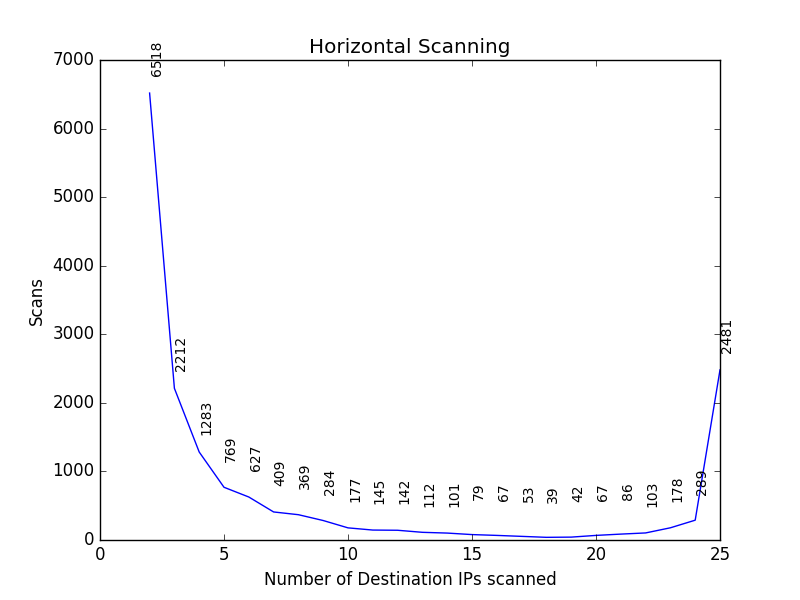
\includegraphics[width=1\linewidth]{images/horizontal_scans_jan_classc}
  \caption{TCP horizontal scanning grouped by same /24 network(without honeypot)}
  \label{fig:test1}
\end{minipage}%
\begin{minipage}{.535\textwidth}
  \centering
  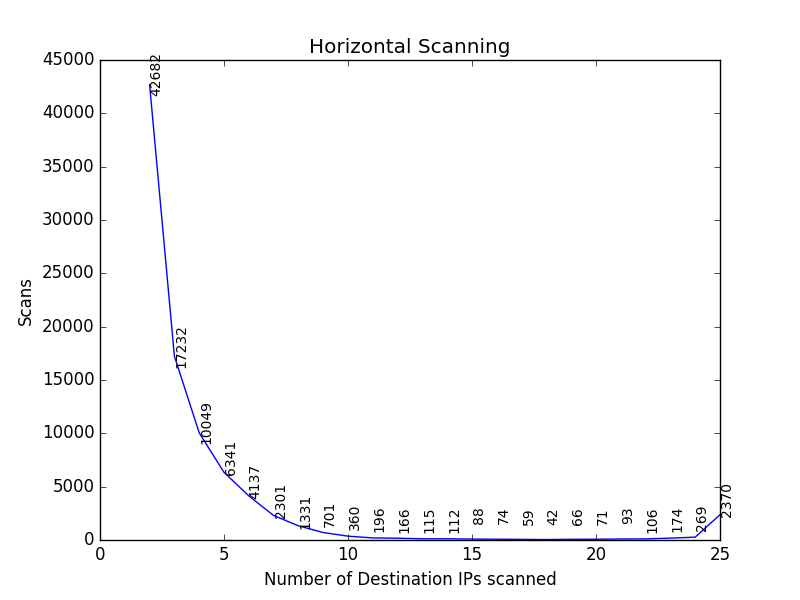
\includegraphics[width=1\linewidth]{images/horizontal_scans_jan_isp}
  \caption{TCP horizontal scanning grouped by same ISP (without honeypot)}
  \label{fig:test2}
\end{minipage}
\end{figure}
\\\\
Figure 7.2 shows the similar graph as explained in the above paragraph, but grouped by same ISP for the initial configuration (without honeypot).
The reason for grouping the horizontal scans by these methods were explained in the section 4.2.
It is clear from Figure 7.2 that, it shows similar behavior as first graph.
Nevertheless, the number of horizontal scans are increased in general for each corresponding horizontal scan size as compared to first graph.
This is due to the fact that, in the second approach, we  consider a very broader perspective by assuming that possibly all attacks from same source come from the same Internet Service Provider (ISP).
So this approach is used to minimize error, but the chances of including the false positives are high.
\begin{figure}[ht]
\captionsetup{justification   = raggedright,
              singlelinecheck = false}
\centering
\begin{minipage}{.535\textwidth}
  \centering
  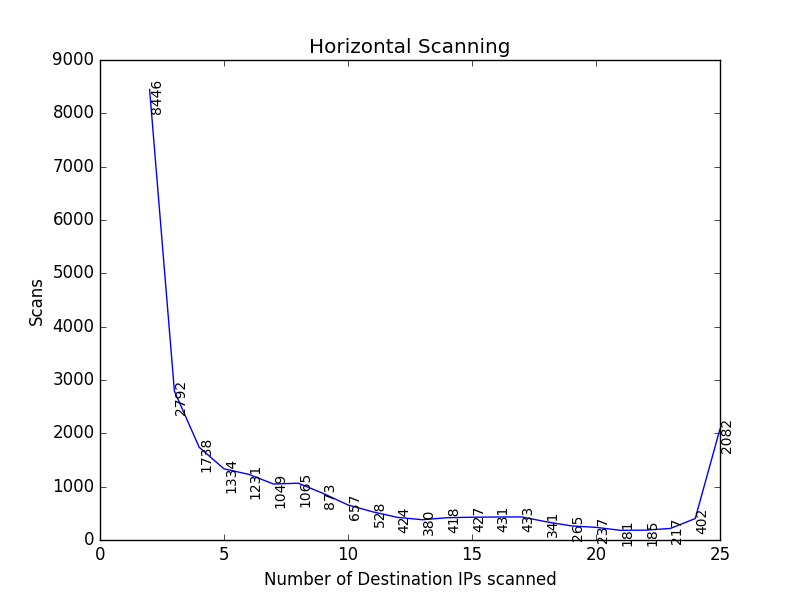
\includegraphics[width=1\linewidth]{images/horizontal_scans_march_classc}
  \caption{TCP horizontal scanning grouped by same /24 network (with honeypot)}
  \label{fig:march_classc}
\end{minipage}%
\begin{minipage}{.535\textwidth}
  \centering
  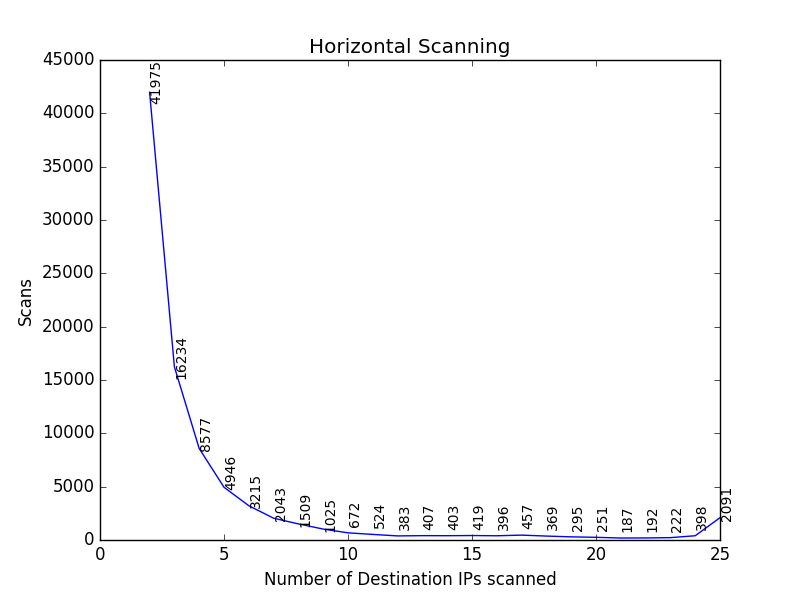
\includegraphics[width=1\linewidth]{images/horizontal_scans_march_isp}
  \caption{TCP horizontal scanning grouped by same ISP (with honeypot)}
  \label{fig:march_isp}
\end{minipage}
\end{figure}
\\\\
Figure 7.3 and Figure 7.4 show the correlation of horizontal scan sizes and number of horizontal scans for the second configuration (with honeypot) grouped by same /24 network and same ISP respectively.
These graphs show similar behavior compared to horizontal scanning graphs plotted by analysing the dataset obtained using network telescope without honeypot.
However it is not very easy to compare the behavior of horizontal scanning with regards to the total number of horizontal scans, as it is larger at second dataset when the scans are grouped by same /24 network but, number of scans is more at first dataset when it is grouped by same ISP.
Examining overall pattern of above mentioned graphs, number of horizontal scans keep reducing when number of distinct destination IP's scanned by scan source increases.
\\\\
Figure 7.5 illustrates the correlation between vertical scans sizes (number of distinct destination ports scanned) and number of vertical scans in TCP port scans for the initial configuration (without honeypot) grouped by same /24 network.
Using this graph and the Table 7.3, we can understand that around 94\% of total vertical scans have been obtained at vertical scan size 2.
It falls dramatically to about 3\% at vertical scan size 3 and it keep decreasing gradually when vertical scan size increases.
Finally number of vertical scans drop to single digit  at vertical scan sizes 79 and 82. 
The graph clearly shows that number of vertical scans get decreasing when the vertical scan size increases.\\\\
Figure 7.6 shows the similar graph as explained in the above paragraph, but grouped by same ISP for the initial configuration (without honeypot).
This graph shows similar behavior as first graph.
However total number of vertical scans have been increased very much compared to first graph and 88\% of the total vertical scans have been shown at vertical scan size 2.
It is interesting to notice that 99\% of the total scans have been obtained before vertical scan size reached 10 in both graphs.
Moreover number of vertical scans is same in both graphs after vertical scan size becomes 10.
These scans were originated from only 4 class C networks such as 185.40.4.0/24, 212.71.238.0/24, 183.3.227.0/24 and 62.210.246.0/24.
In the second graph false positives might have included in the initial values of vertical scan size since difference between number of vertical scans in the first and second graphs keep reducing when vertical scan size increases.
\\\\
\begin{figure}[p]
\centering
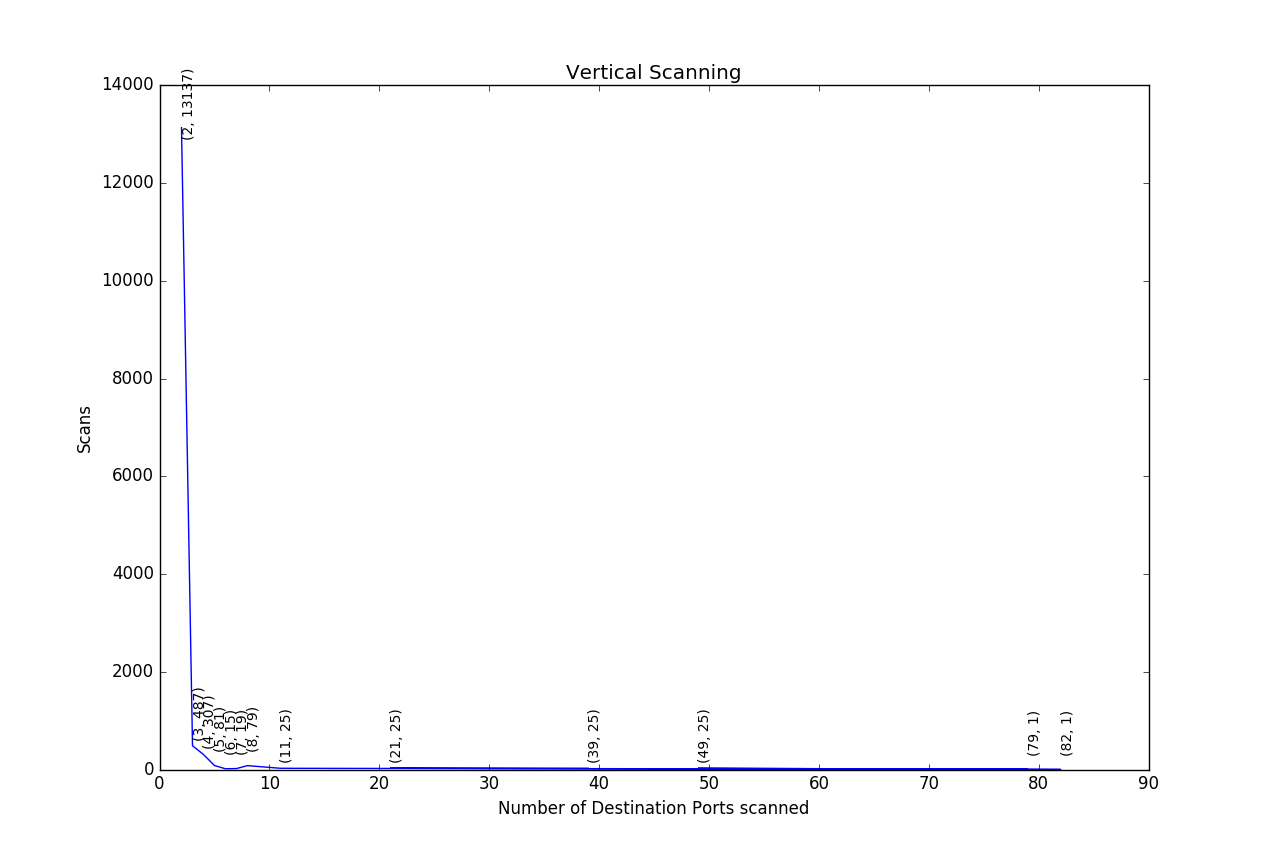
\includegraphics[width=15cm,height=9cm]{images/vertical_scans_jan_classc}
\caption{ TCP vertical scanning grouped by same /24 network (without honeypot)}
\centering
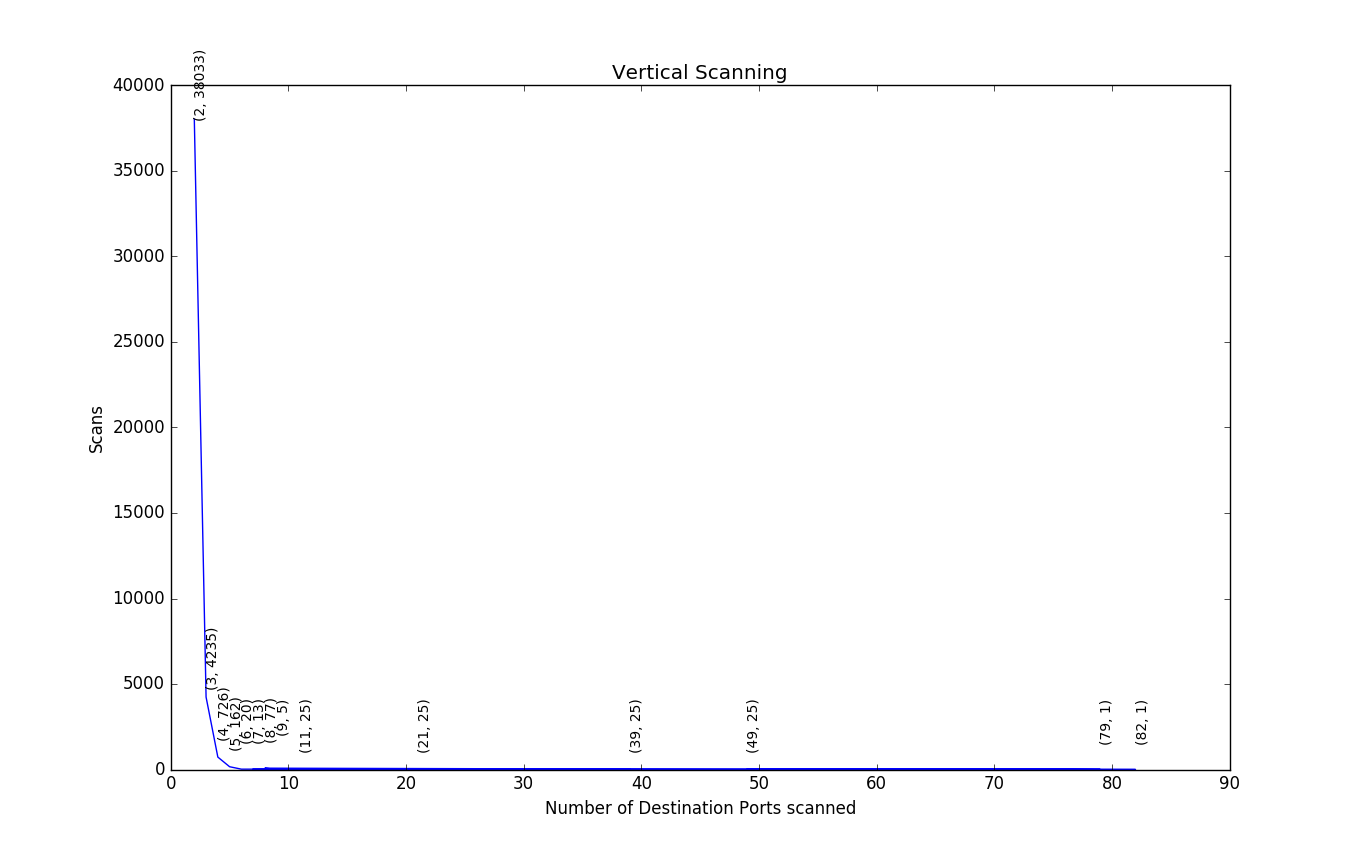
\includegraphics[width=15cm,height=9cm]{images/vertical_scans_jan_isp}
\caption{ TCP vertical scanning grouped by same ISP (without honeypot)}
\end{figure}
\begin{figure}[p]
\centering
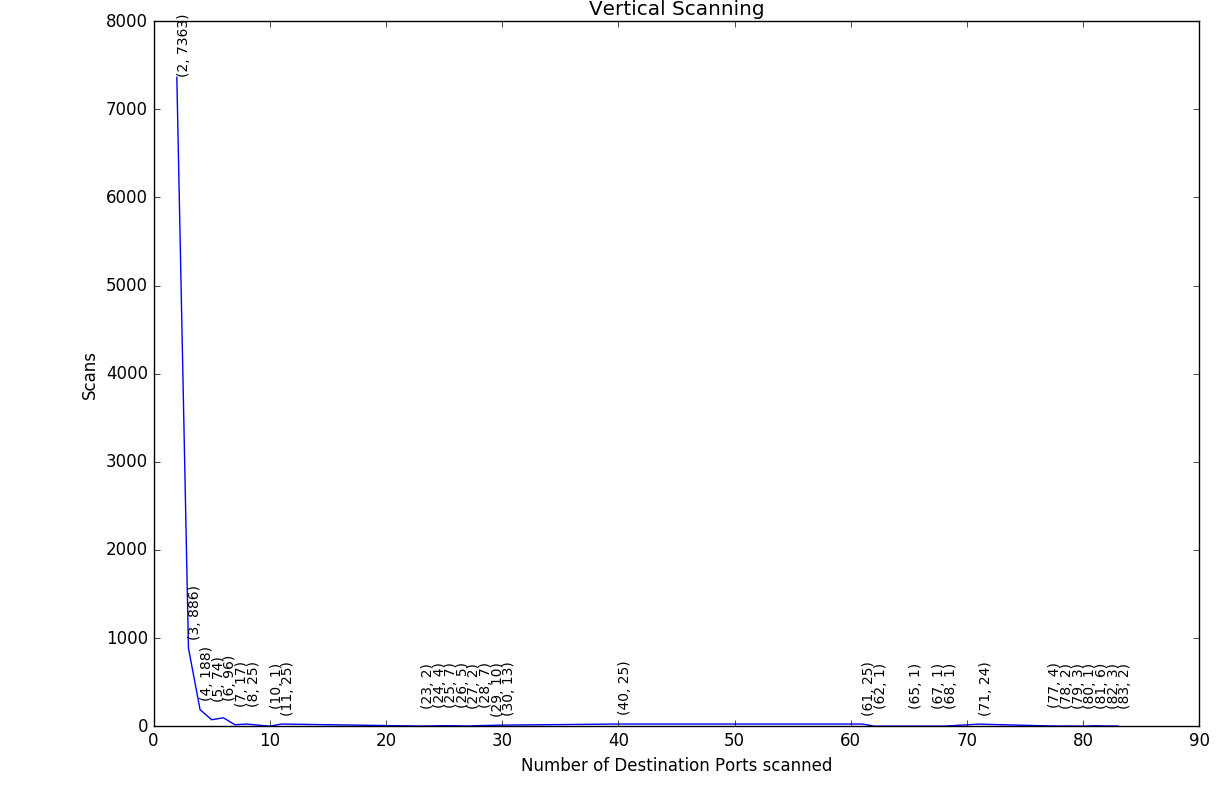
\includegraphics[width=15cm,height=9cm]{images/vertical_scans_march_classc}
\caption{ TCP vertical scanning grouped by same /24 network (with honeypot)}
\centering
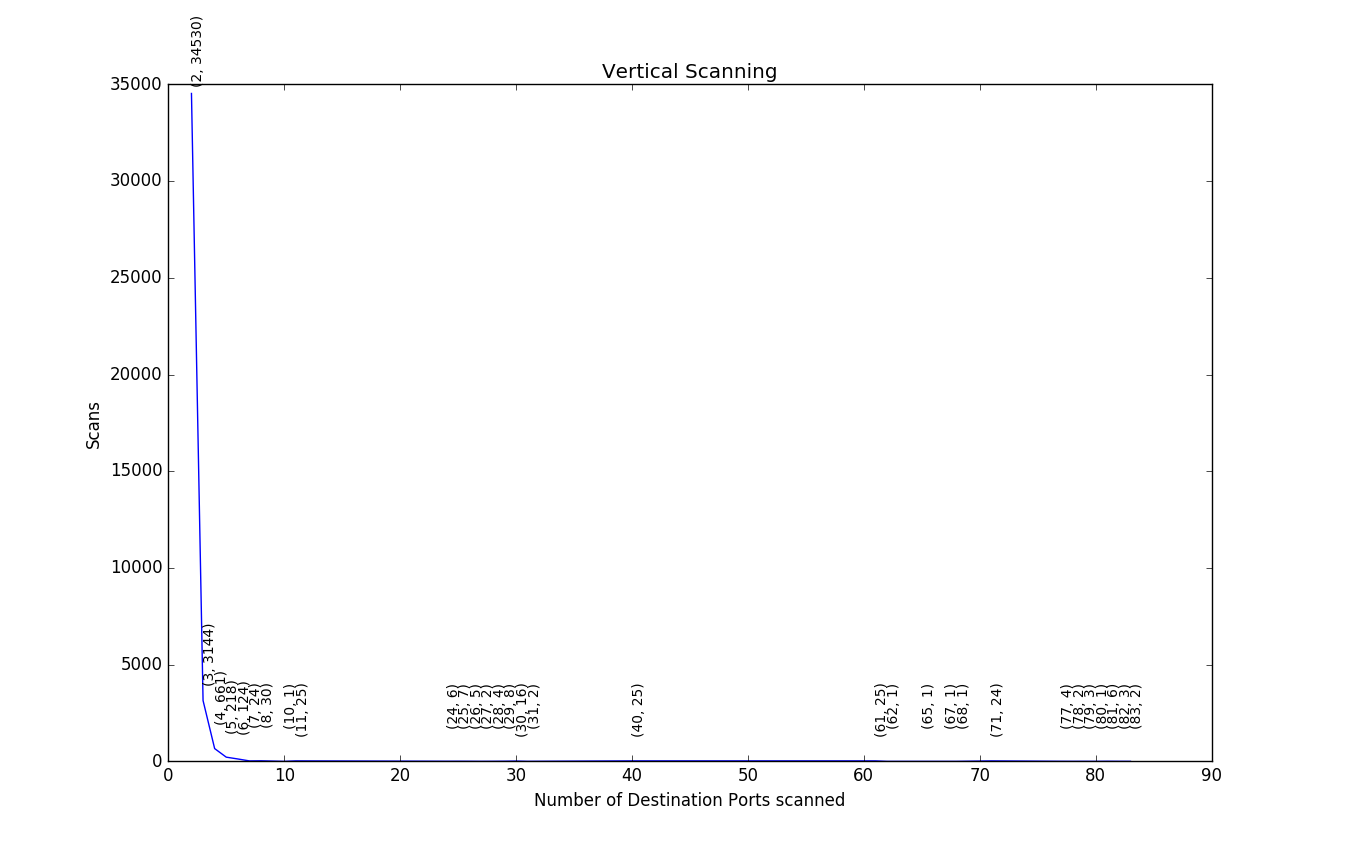
\includegraphics[width=16.5cm,height=9cm]{images/vertical_scans_march_isp}
\caption{ TCP vertical scanning grouped by same ISP (with honeypot)}
\end{figure}
\newpage
\noindent
Figure 7.7 and Figure 7.8 show the correlation of vertical scans sizes and number of vertical scans in TCP port scans for the second configuration (with honeypot) grouped by same /24 network and same ISP respectively. 
These graphs show similar behavior compared to vertical scanning graphs plotted by analysing the dataset obtained using network telescope without honeypot. 
In the Figure 7.7, around 83\% of total vertical scans have been obtained at vertical scan size 2 and it falls to around 6\% at vertical scan size 3.
As similar to graph explained in previous paragraph, number of vertical scans keep decreasing gradually when vertical scan size increases.
In the Figure 7.8, total number of vertical scans have been increased very much compared to first graph.
Similar to vertical scanning graphs obtained using first dataset, number of vertical scans is same in both graphs after vertical scan size becomes 10.
Vertical scans which are targeted on more than 10 destination ports are coming from mainly four countries: China, United States, France and Switzerland.
Moreover these scans are originated from only 6 class C networks such as 113.240.250.0/24 , 69.64.33.0/24, 222.186.34.0/24, 163.172.99.0/24, 193.138.215.0/24 and 173.254.236.0/24 at multiple times during this time span.\\\\ 
From the above mentioned four graphs,  we can see that there are small number
of large scans, with the size distribution being dominated by small scans.
However, number of large scans in the graphs from the second configuration (with honeypot) have been increased in general compared to graphs from the first configuration.
In addition to that, number of different vertical scan sizes have been also increased in the graphs obtained at second configuration compared to graphs from the first configuration.
\subsubsection{Horizontal and Vertical Scanning in UDP Port Scans}
Table 7.5 illustrates number of horizontal and vertical scans in UDP scans for two datasets and its counts. 
Number of horizontal and vertical scanning in UDP port scans are less compare to the corresponding values in TCP port scans.
Moreover, similar to Table 7.3, horizontal and vertical scanning counts are high when it is grouped by same ISP compared to when it is grouped by same /24 network in both first and second configuration.
\begin{table}[t!]
    \centering
    \resizebox{\columnwidth}{!}{%
    \begin{tabular}{c|c|c|c|}
    \hline
    \multicolumn{1}{ |c| }{Network Telescope Configuration}& Grouping & Number of Horizontal scans & Number of Vertical scans  \\ \cline{1-4}
    \multicolumn{1}{ |c  }{\multirow{2}{*}{Without Honeypot} } &
    \multicolumn{1}{ |c| }{same /24 network} & 7801 & 1715  \\ \cline{2-4}
    \multicolumn{1}{ |c  }{}                        &
    \multicolumn{1}{ |c| }{same ISP} & 11130 & 2612   \\ \cline{1-4}   
    \multicolumn{1}{ |c  }{\multirow{2}{*}{With Honeypot} } &
    \multicolumn{1}{ |c| }{same /24 network} & 9080 & 1158 \\ \cline{2-4}
    \multicolumn{1}{ |c  }{}  &
    \multicolumn{1}{ |c| }{same ISP} & 10794 & 2318   \\ \cline{1-4}   
    \end{tabular}
    }
    \caption{Number of Horizontal and Vertical scans in UDP Port Scans for Two Datasets and its Counts}
\end{table}
\begin{figure}
\captionsetup{justification   = raggedright,
              singlelinecheck = false}
\centering
\begin{minipage}{.535\textwidth}
  \centering
  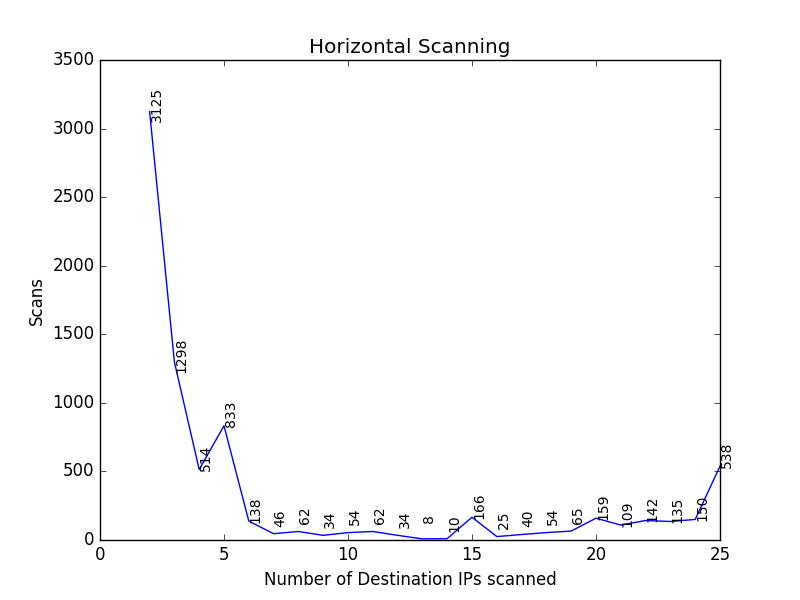
\includegraphics[width=1\linewidth]{images/horizontalscan_udp_classc}
  \caption{UDP horizontal scanning grouped by same /24 network(without honeypot)}
  \label{fig:horizontalscanningudpsameclassc}
\end{minipage}%
\begin{minipage}{.535\textwidth}
  \centering
  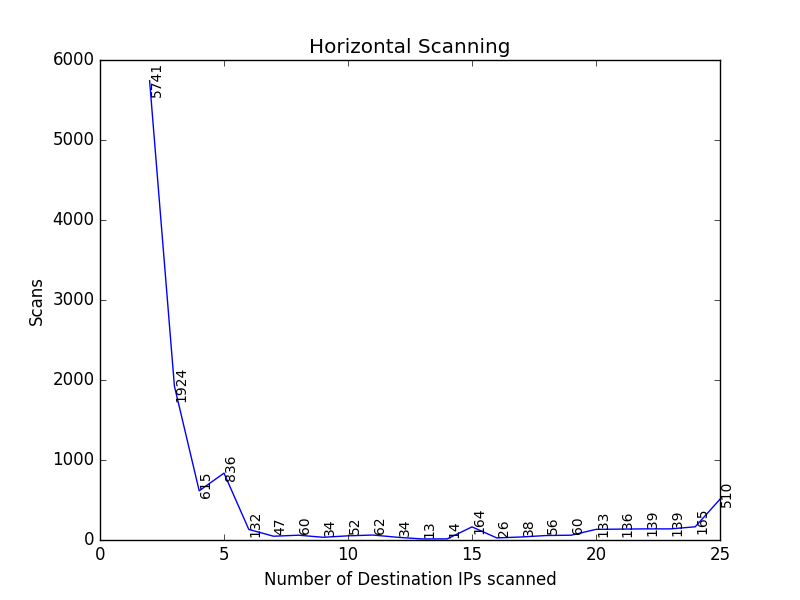
\includegraphics[width=1\linewidth]{images/horizontalscan_udp_isp_first}
  \caption{UDP horizontal scanning grouped by same ISP (without honeypot)}
  \label{fig:horizontalscanningudpsameisp}
\end{minipage}
\end{figure}
\\\\
Figure 7.9 and Figure 7.10 show the correlation of horizontal scan sizes and number of horizontal scans in UDP port scans for first configuration (without honeypot) grouped by same /24 network and same ISP respectively.
Overall, similar to behavior of  horizontal scanning graphs for TCP port scans shown in Figure 7.1 and 7.2, the number of horizontal scans are decreased in respect to increase of number of destination IPs scanned.
However, number of horizontal scans are less in general for each corresponding horizontal scan size as compared to graphs in Figure 7.1 and 7.2.
\begin{figure}[h!]
\captionsetup{justification   = raggedright,
              singlelinecheck = false}
\centering
\begin{minipage}{.535\textwidth}
  \centering
  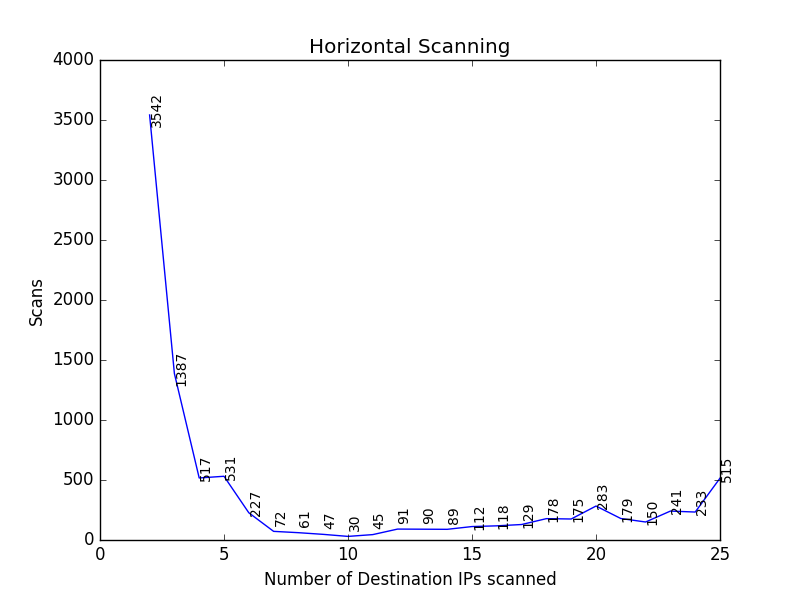
\includegraphics[width=1\linewidth]{images/horizontalscan_udp_classc_honeypot}
  \caption{UDP horizontal scanning grouped by same /24 network(with honeypot)}
  \label{fig:horizontalscanningudpsameclasscwithhoneypot}
\end{minipage}%
\begin{minipage}{.535\textwidth}
  \centering
  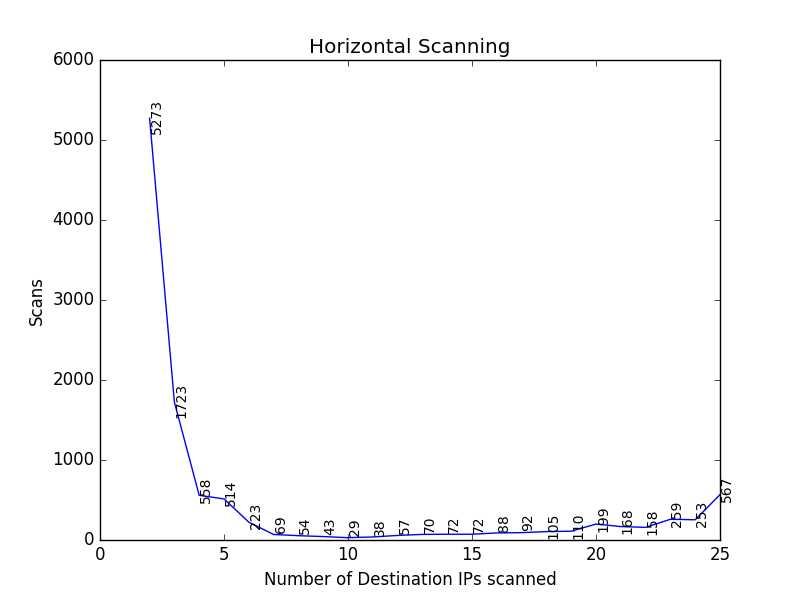
\includegraphics[width=1\linewidth]{images/horizontalscan_udp_isp_honeypot}
  \caption{UDP horizontal scanning grouped by same ISP (with honeypot)}
  \label{fig:horizontalscanningudpsameispwithhoneypot}
\end{minipage}
\end{figure}
\\\\
Figure 7.11 and Figure 7.12  show the correlation of horizontal scan sizes and number of horizontal scans in UDP port scans for the second configuration (with honeypot) grouped by same /24 network and same ISP respectively.
These graphs also show similar behavior compared to  horizontal scanning graphs for TCP port scans shown in Figure 7.3 and 7.4.
Nevertheless, number of horizontal scans are less in general for each corresponding horizontal scan size as compared to graphs in Figure 7.3 and 7.4.
Nevertheless, number of horizontal scans are less in general for each corresponding horizontal scan size as compared to graphs in Figure 7.3 and 7.4.
\begin{figure}[p]
\centering
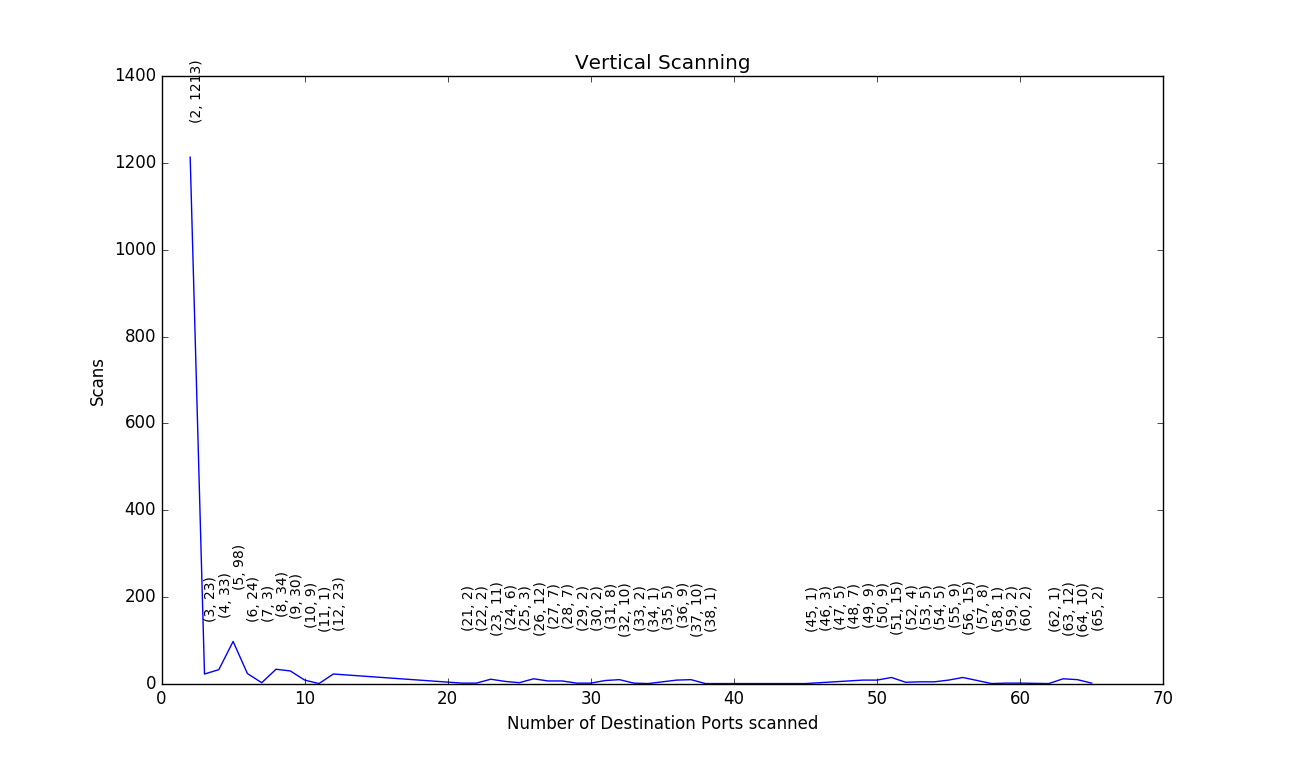
\includegraphics[width=15cm,height=9cm]{images/verticalscan_udp_classc}
\caption{ UDP vertical scanning grouped by same /24 network (without honeypot)}
\centering
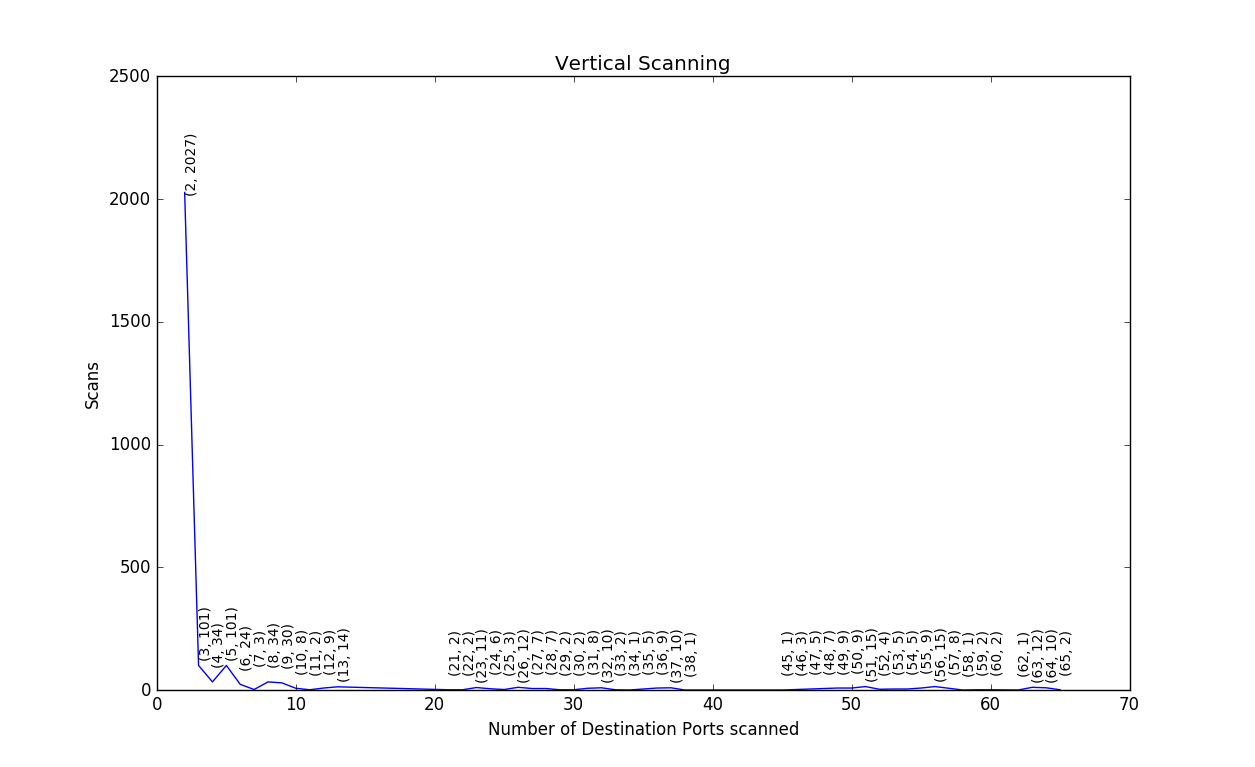
\includegraphics[width=15cm,height=9cm]{images/verticalscan_udp_isp_first}
\caption{ UDP vertical scanning grouped by same ISP (without honeypot)}
\end{figure}
\\\\
Figure 7.13 and Figure 7.14 show the correlation of vertical scans sizes and number of vertical scans in UDP scans for the first configuration (without honeypot) grouped by same /24 network and same ISP respectively.
From Figure 7.13 and Table 7.5, we can understand that around 71\% of total vertical scans have been obtained at vertical scan size 2.
In Figure 7.14, around 78\% of total vertical scans have been obtained at vertical scan size 2.
Similar to graphs plotted in Figure 7.5 and 7.6, these graphs also show that number of vertical scans get decreasing in general when the vertical scan size increases.
Moreover, it is interesting to notice that number of vertical scans is same in both graphs after vertical scan size 20. 
It is because all these port scans were generated from only one source IP address which is 104.193.11.107.
From the explanation given for Figure 7.5 and 7.6,  it is understood that this IP address (104.193.11.107) did not participate in TCP vertical scans which target on more than 20 destination ports during the same time period.
\begin{figure}[p]
\centering
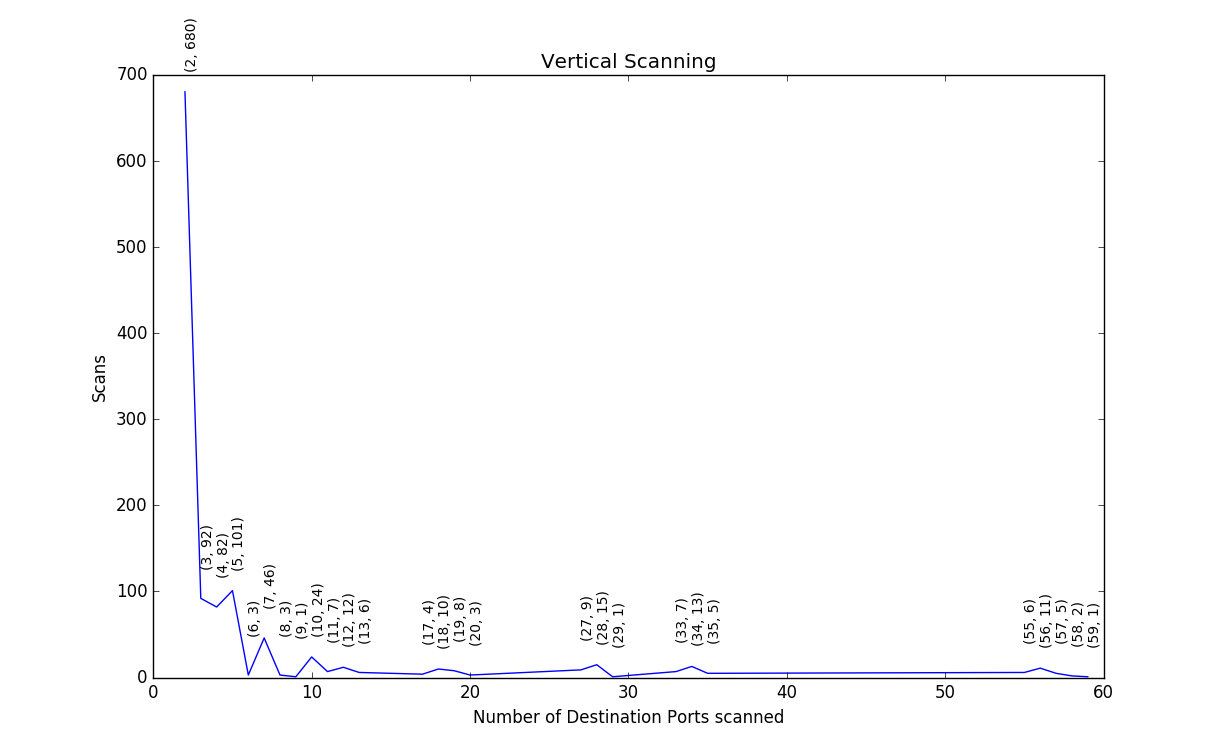
\includegraphics[width=15cm,height=9cm]{images/verticalscan_udp_classc_honeypot}
\caption{ UDP vertical scanning grouped by same /24 network (with honeypot)}
\centering
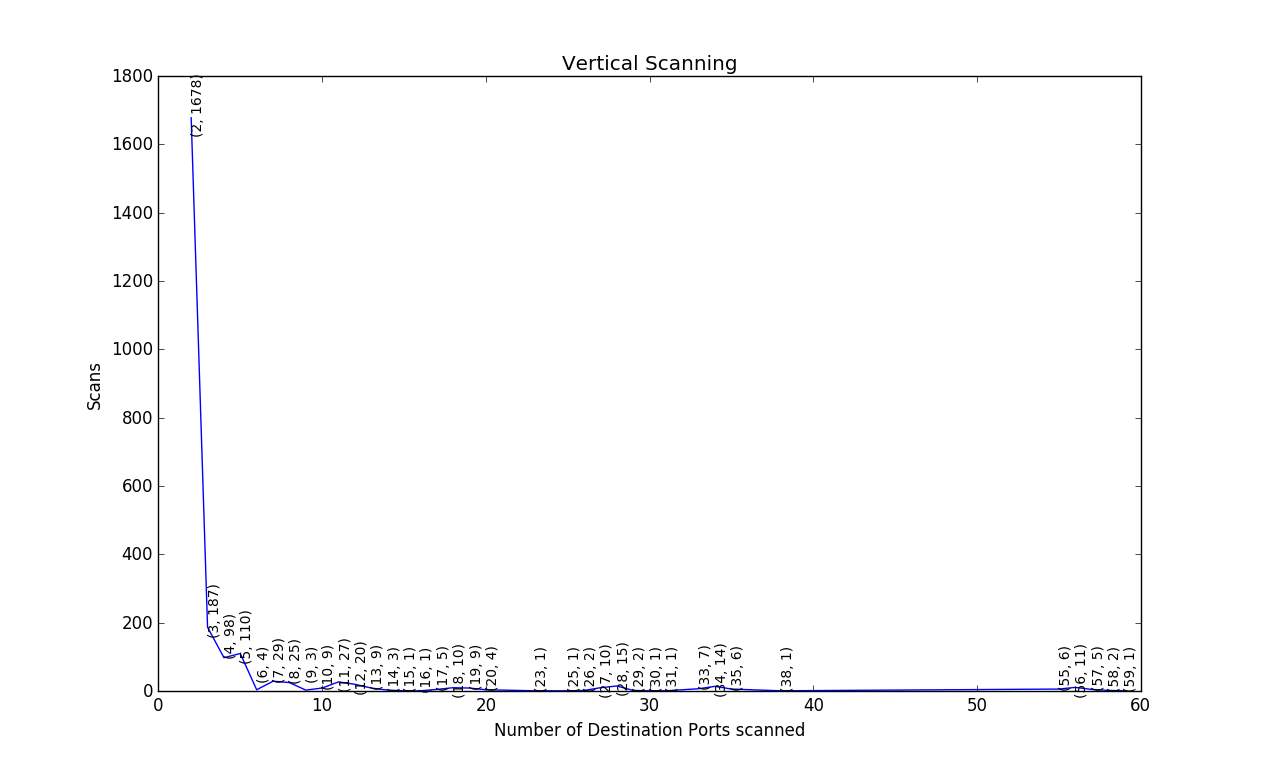
\includegraphics[width=16.5cm,height=9cm]{images/verticalscan_udp_isp_honeypot}
\caption{ UDP vertical scanning grouped by same same ISP (with honeypot)}
\end{figure}
\\\\
Figure 7.15 and Figure 7.16 show the correlation of vertical scans sizes and number of vertical scans in UDP port scans for the second configuration (with honeypot) grouped by same /24 network and same ISP respectively.
These graphs show similar behavior compared to  vertical scanning graphs for TCP port scans shown in Figure 7.7 and 7.8.
Similar to analysis results obtained in previous paragraph, more than half amount of total vertical scans have been received at vertical scan size 2 for both graphs plotted in Figure 7.15 and 7.16.
However, number of vertical scans which is targeted on more than 20 destination ports are less during second configuration compared to same value in first configuration.
While comparing the source IPs targeted on more than 20 destination ports for TCP and UDP vertical scans, we can see that
source IPs who perform large scans at TCP and UDP ports are different.
From the graphs plotted for the analysis of vertical scans in UDP port scans, we can understand that there are small number of large scans, with the size distribution being dominated by small scans as similar to the results of TCP port scans. 
\subsection{Target Ports}
The popularity of target ports for TCP and UDP packets was another metric we evaluated during the analysis of dataset obtained from first and second configuration.
We analysed captured packets from these two configurations and compared the behavior of port scan activity based on targeted ports.\\\\
\newpage 
\noindent
In the first dataset, out of total 65536 port numbers, only  913 TCP ports were scanned at least once during this time span.
As some of the ports were scanned only once during this time span, around 93\% of the ports were scanned many more times during this period.
Table 7.5 lists the top 20 most actively scanned TCP ports, the corresponding services and some related statistics from dataset obtained at first configuration.
We can see that more than half of the total TCP scans were targeted on port 23.
Port 22 was scanned more than 6\% of the total port scans.
 \begin{table}[t!]
    \centering
    \scalebox{0.7}{
    \begin{tabular}{ |c|c|c|c| }
     \hline
     \textbf{Port Number} & \textbf{Number Of Hits} & \textbf{Percentage of Total} & \textbf{Port Services} \\
     \hline
     23 & 371626 & 51.7 & Telnet\\ 
     \hline
     22 & 52303 & 6.5 & SSH \\ 
     \hline
    7547 & 47551 & 5.9 & \makecell{TR-069 -Application layer protocol for  \\ remote management of end-user devices.}\\
    \hline
    2323 & 32002 &  4.5 & \makecell{3d-nfsd - Special file system for\\ controlling Linux NFS server} \\ 
    \hline
    6789 & 34422 & 4.3  & IBM db2 web control center\\
    \hline
    23231 & 32053 & 4  & Unassigned\\ 
    \hline
    5358 & 27571 &  3.4 &wsdapi-s - Web Services for Devices Secured port\\ 
    \hline
    1433 & 18936 &  2.4 &SMC-HTTPS\\ 
    \hline
    443 & 15792 &  2.1 &HTTP protocol over TLS/SSL\\ 
    \hline
    37777 &  10216 &  1.2 &Digital Video Recorder hardware\\ 
    \hline
    3389 & 9247&  1.1 & \makecell{Microsoft Terminal Server (RDP) officially \\ registered as Windows Based Terminal (WBT)}\\
    \hline
    80 & 6976 & 0.87 &HTTP\\
    \hline
    8080 &  5826&  0.73 &HTTP Alternate\\ 
    \hline
    3306 & 5229 & 0.65 &Microsoft Directory Services\\ 
    \hline
    2222 &  4720&  0.59 &Rockwell CSP2\\ 
    \hline
    1099 &  2196&  0.27 &RMI Registry\\ 
    \hline
    445 &  1921 & 0.24 &Microsoft Directory Services\\ 
    \hline
    5900 &  1856&  0.23 &Virtual Network Computing (VNC)-  remote
control program\\ 
    \hline
    21 & 1564 & 0.19 &FTP - File Transfer Protocol\\
    \hline
    81 & 1480 & 0.18 & HTTP Alternate\\ 
    \hline
    \end{tabular}
    }
    \caption{Top 20: Most Actively Scanned TCP Ports and their Functions without Honeypot}
\end{table}
\begin{table}[t!]
    \centering
    \scalebox{0.7}{
    \begin{tabular}{ |c|c|c|c| } 
     \hline
    \textbf{Port Number} & \textbf{Number Of Hits} & \textbf{Percentage of Total} & \textbf{Port Services} \\
     \hline
     23 & 315374 & 39.6 & Telnet\\ 
     \hline
     22 & 120980 & 15.2 & SSH \\ 
     \hline
    5358 & 70943 & 8.9 &wsdapi-s - Web Services for Devices Secured port\\
    \hline
    7547 & 49162 & 6.1 & \makecell{TR-069 -Application layer protocol for  \\ remote management of end-user devices.}\\
    \hline
    2323 & 23719 & 2.9& \makecell{3d-nfsd - Special file system for\\ controlling Linux NFS server} \\ 
    \hline
    443 & 17898 & 2.2 &HTTP protocol over TLS/SSL\\ 
    \hline
    80 & 14815 & 1.8 &HTTP\\
    \hline
     3389 & 11036 & 1.3 & \makecell{Microsoft Terminal Server (RDP) officially \\ registered as Windows Based Terminal (WBT)}\\
    \hline
    3306 & 8980 & 1.1 &Microsoft Directory Services\\ 
    \hline
    8080 &  8413 & 1.05 &HTTP Alternate\\ 
    \hline
    1433 & 7702 & 0.96 &SMC-HTTPS\\ 
    \hline
    2222 & 6181 & 0.77 & Rockwell CSP2\\
    \hline
    445 &   3078 & 0.38 &Microsoft Directory Services\\ 
    \hline
     21 & 3075 & 0.38 &FTP - File Transfer Protocol\\
    \hline
    81 & 2870 & 0.36 & HTTP Alternate\\ 
    \hline
    5900 &  2715 & 0.34 & Virtual Network Computing (VNC)- remote
    control program\\
    \hline
    25 & 2471 & 0.31 & Simple Mail Transfer Protocol (SMTP)\\
    \hline
    88 & 2185 & 0.27 & Kerberos Key Distribution Center (KDC) server\\
    \hline
    6789 & 1867 & 0.23  & IBM db2 web control center\\
    \hline
    3390 & 1798 & 0.22 & Trojans\\ 
    \hline
    \end{tabular}
    }
    \caption{Top 20: Most Actively Scanned TCP Ports and their Functions with Honeypot}
\end{table}
Most of the ports in the Table 7.5 run a service that can be exploited by attackers except port 23231 in which no popular service is assigned on.
When we studied more extensively about port 23231, we understand that the large number of port scans are due to Mirai vulnerability scanning activity.
Mirai vulnerability scanner scans the IP addresses to check if the target network hosts a device vulnerable to Mirai injection attacks \cite{hallman2017ioddos}.
Since there is no active service reside on port 23231, Figure 7.17 clearly shows that TCP connection includes only two packets and port 23231 is closed.
Moreover it shows that, there is no actual data being transferred between source and target system. 
\begin{figure}[ht]
\centering
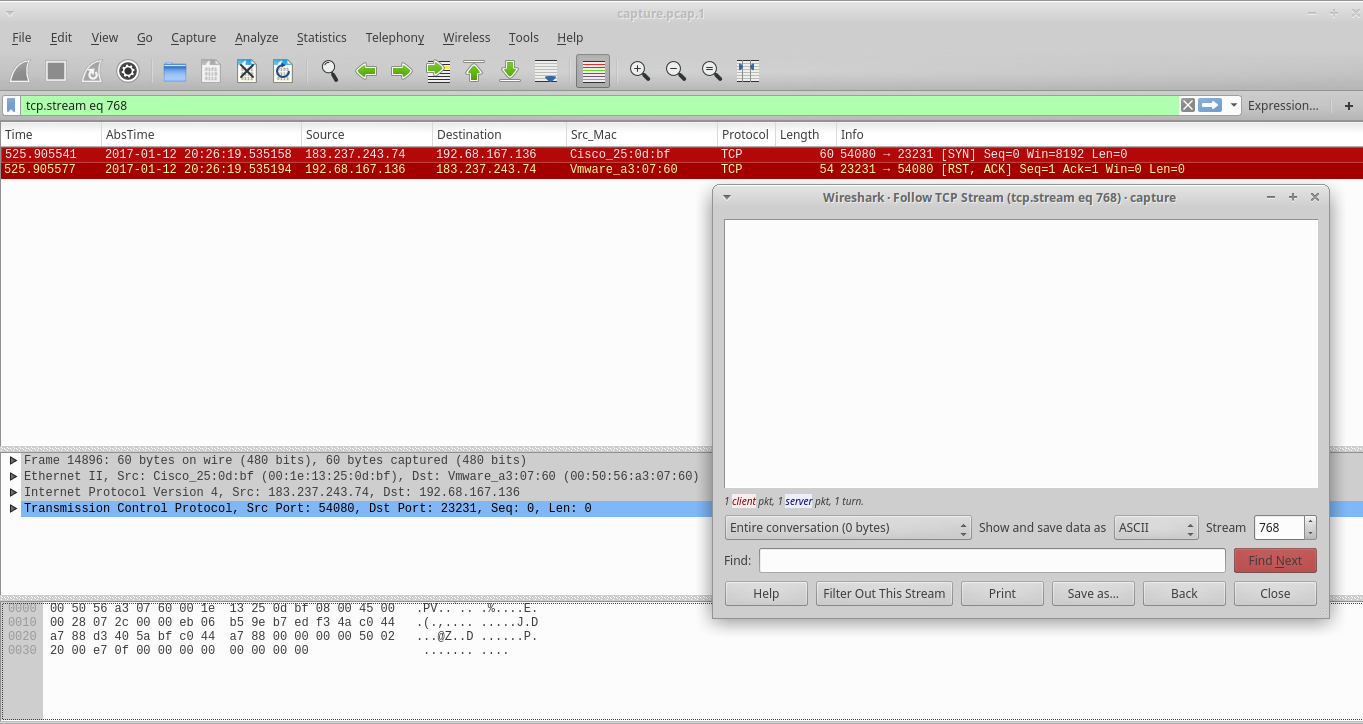
\includegraphics[width=16cm, height=10cm]{images/23231port.png}
\caption{TCP stream of port scan targeted on port 23231 shows that port is closed and there is no actual data being transferred between source and target system }
\end{figure}
\\\\
In the second dataset, out of total 65536 port numbers, 1295 TCP ports were scanned at least once during this time span.
Comparing the number of ports scanned at first and second configuration, there is 41\% of increase in second stage.
This is due to more number of large scans in the second configuration, thus more number of ports are scanned as we discussed while explaining the Figure 7.7.
Around 92\% of the ports were scanned many more times during this period and amount of scans targeted on ports only once are very less. 
Table 7.6 lists the top 20 most actively scanned TCP ports, the corresponding services and some related statistics from dataset obtained at second configuration.
We can see that nearly 40\% of the total TCP scans were targeted on port 23.
Port 22 was scanned more than 15\% of the total port scans.
All top 20 ports are well known for running some services which are vulnerable for attacks.\\\\
We also analysed most actively scanned UDP ports as part of thesis work.
In the first dataset, out of total  65536 UDP ports, 825 UDP ports were scanned at least once during this time period.
Around 81\% of the UDP ports were scanned multiple times during this time period.
While during second configuration, 2249 UDP ports were scanned at least once.
However only 19\% of these ports were scanned multiple times during this period.
Comparing the number of TCP and UDP ports scanned at first and second configuration, we can see that a large percentage of increase in scanned ports at dataset obtained using network telescope with honeypot.
\begin{table}[t!]
    \centering
    \scalebox{0.7}{
    \begin{tabular}{ |c|c|c|c| } 
     \hline
     \textbf{Port Number} & \textbf{Number Of Hits} & \textbf{Percentage of Total} & \textbf{Port Services} \\
     \hline
     1900 & 23123 & 24.9& UPnP Simple Service Discovery Protocol (SSDP)\\
     \hline
     5060 & 22061 & 23.7 & Session Initiation Protocol (SIP)\\
     \hline
     161 & 5283 & 5.6 & SNMP\\
     \hline
     53413 & 4043 & 4.3 & Netis Router Backdoor\\
     \hline
     123 & 3528 & 3.8 & Network Time Protocol(NTP)\\
     \hline
    53 & 2739 & 2.9& DNS\\
    \hline
    2425 & 2427 & 2.6 & Fujitsu App Manager\\
    \hline
    137 & 1699 & 1.8 & Netbios\\
    \hline
    1434 & 1334 & 1.4 & Microsoft SQL Server\\
    \hline
    19 & 1000 & 1.07 & Character Generator Protocol(CHARGEN)\\
    \hline
    \end{tabular}
    }
    \caption{Top 10: Most Actively Scanned UDP Ports and their Functions without Honeypot}
\end{table}
\begin{table}[t!]
    \centering
    \scalebox{0.7}{
    \begin{tabular}{ |c|c|c|c| } 
     \hline
     \textbf{Port Number} & \textbf{Number Of Hits} & \textbf{Percentage of Total} & \textbf{Port Services} \\
     \hline
     5060 & 47292 & 42.8 & Session Initiation Protocol (SIP)\\
     \hline
     1900 &16463 & 14.9 & UPnP Simple Service Discovery Protocol (SSDP)\\
     \hline
     161 & 6728 & 6.1 & SNMP\\
     \hline
     53413 & 5451 & 4.9 & Netis Router Backdoor\\
    \hline
    123 & 3752 & 3.4 &Network Time Protocol(NTP)\\ 
     \hline
     53 & 3402 & 3.08 & DNS\\
    \hline
    137 & 1870 & 1.6 & Netbios\\
    \hline
    1434 & 1457 & 1.3 & Microsoft SQL Server\\
    \hline
    2425 & 1348 & 1.2 & Fujitsu App Manager\\
    \hline
    19 &1279 &1.1& Character Generator Protocol(CHARGEN)\\ 
    \hline
    \end{tabular}
    }
    \caption{Top 10: Most Actively Scanned UDP Ports and their Functions with Honeypot}
\end{table}
\\\\
Table 7.7 and Table 7.8 illustrate most actively scanned UDP ports and its function from dataset obtained at first and second configuration respectively.
All the top 10 ports are same in both Tables which show that these ports were most actively scanned ports irrespective of time period at which port scans were detected.
\subsection{Relationship between Traffic and Time of the Day}
Time distribution of port scan traffic for top 5 countries who participated in scanning activity was yet another metric we evaluated during the analysis of dataset obtained from first and second configuration.
We plotted a graph which shows the relationship between traffic rate and the time of the day for each country, to check if port scanning is a constant activity throughout the day or attackers are more interested in a particular time of the day to execute port scanning.\\\\
Figure 7.18 shows top 5 countries who participated in TCP port scanning activity and its traffic rate based on the local time of the source of attack from first configuration.
It is clear from the graph that, port scanning activity is a constant activity and graph does not show a correlation between traffic and time of the day.
In addition to that, Table 7.9 lists top 5 countries which involved in TCP port scanning activity at first configuration.  
\begin{figure}[p]
\centering
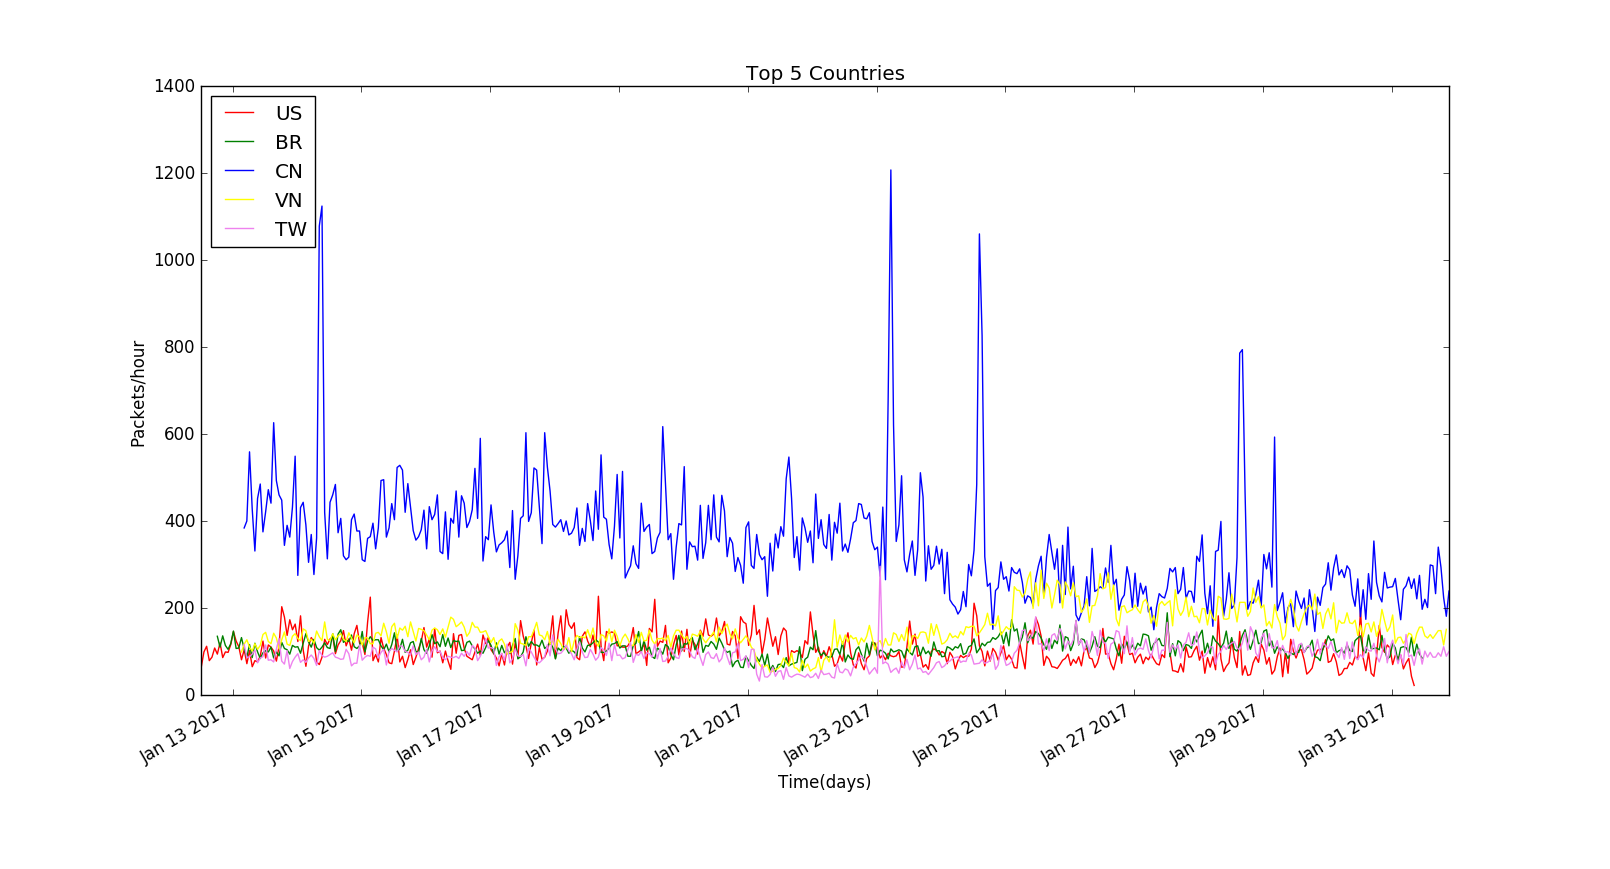
\includegraphics[width=16cm, height=9cm]{images/top5_countries_tcp_withouthoneypot1.png}
\caption{Top 5 countries participated in TCP port scanning activity and its traffic rate (first configuration)}
\centering
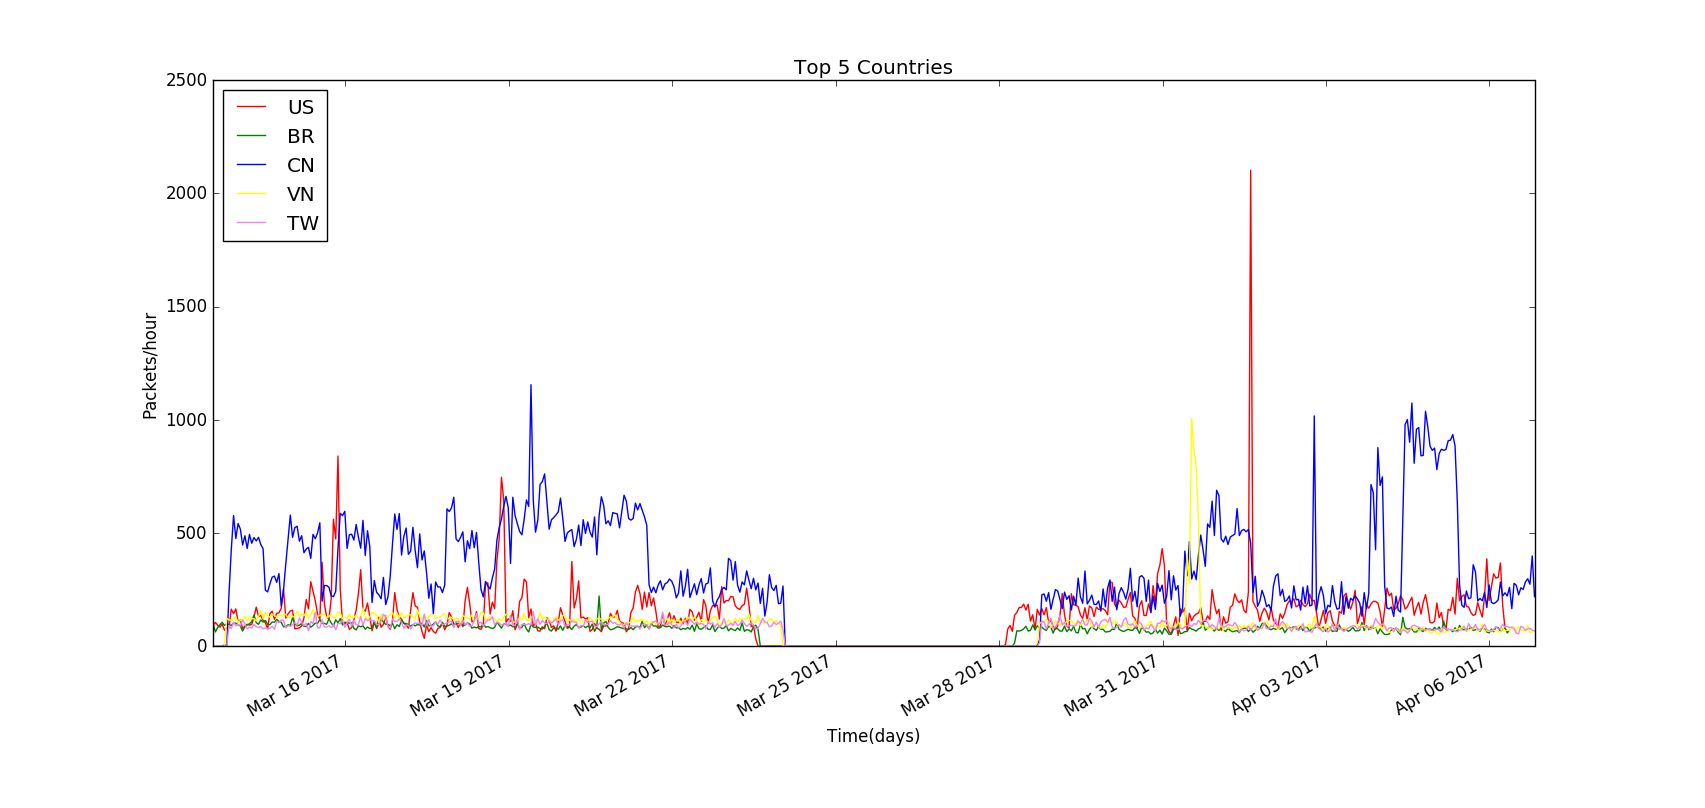
\includegraphics[width=16cm, height=9cm]{images/top5countries_tcp_march2.png}
\caption{Top 5 countries participated in TCP port scanning activity and its traffic rate (second configuration)}
\end{figure}
\begin{table}[t!]
    \centering
    \scalebox{0.7}{
    \begin{tabular}{ |c|c|c| } 
     \hline
     \textbf{Countries} & \textbf{Number of Scans} & \textbf{\% Total Scans} \\ 
     \hline
     China (CN) & 158366 & 19.9\\
     Vietnam (VN) & 68016 & 8.5\\
     United States (US) &  61874 & 7.7\\
     Brazil (BR)& 52167 & 6.5\\
     Taiwan (TW) & 42142 & 5.2\\
     \hline
    \end{tabular}
    }
    \caption{Top 5 countries participated in TCP port scanning activity at first configuration}
\end{table}
\begin{table}[t!]
    \centering
    \scalebox{0.7}{
    \begin{tabular}{ |c|c|c| } 
     \hline
     \textbf{Countries} & \textbf{Number of Scans} & \textbf{\% Total Scans} \\ 
     \hline
     China (CN) & 180169 & 22.3\\
     United States (US)& 93276 & 11.5\\
     Vietnam (VN) & 52076 & 6.4\\
     Brazil (BR) & 43279 & 5.3\\
     Taiwan (TW)& 40866 & 5.1\\
     \hline
    \end{tabular}
    }
    \caption{Top 5 countries participated in TCP port scanning activity at second configuration}
\end{table}
\\\\
Figure 7.19 shows top 5 countries who participated in TCP port scanning activity and its traffic rate based on the local time of the source of attack from second configuration.
Graph shows a similar behavior to the Figure 7.18 and port scanning is a constant activity in the second configuration also.
Table 7.10 illustrates top 5 countries which are involved in TCP port scanning activity at second configuration.
From Table 7.9 and 7.10, it is evident that top countries which involved in TCP port scans at both configurations are same.
\begin{figure}[p]
\centering
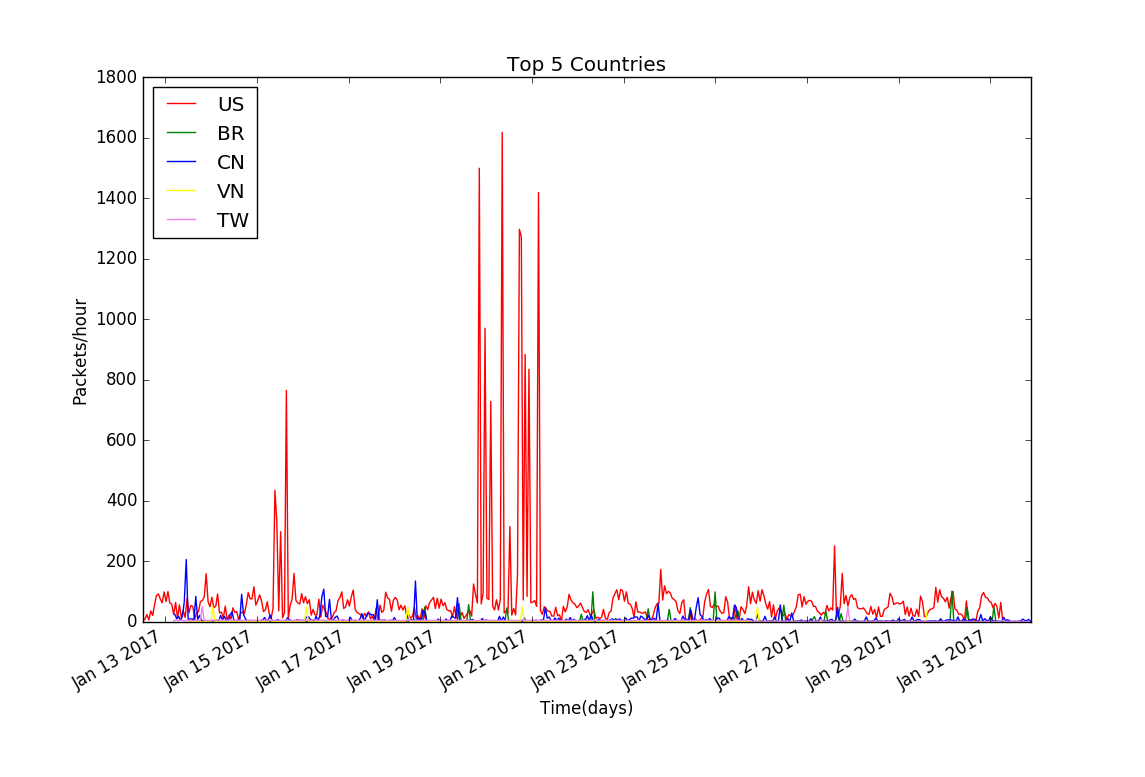
\includegraphics[width=15cm, height=9cm]{images/top5countries_udp_first.png}
\caption{Top 5 countries participated in UDP port scanning activity and its traffic rate (first configuration)}
\centering
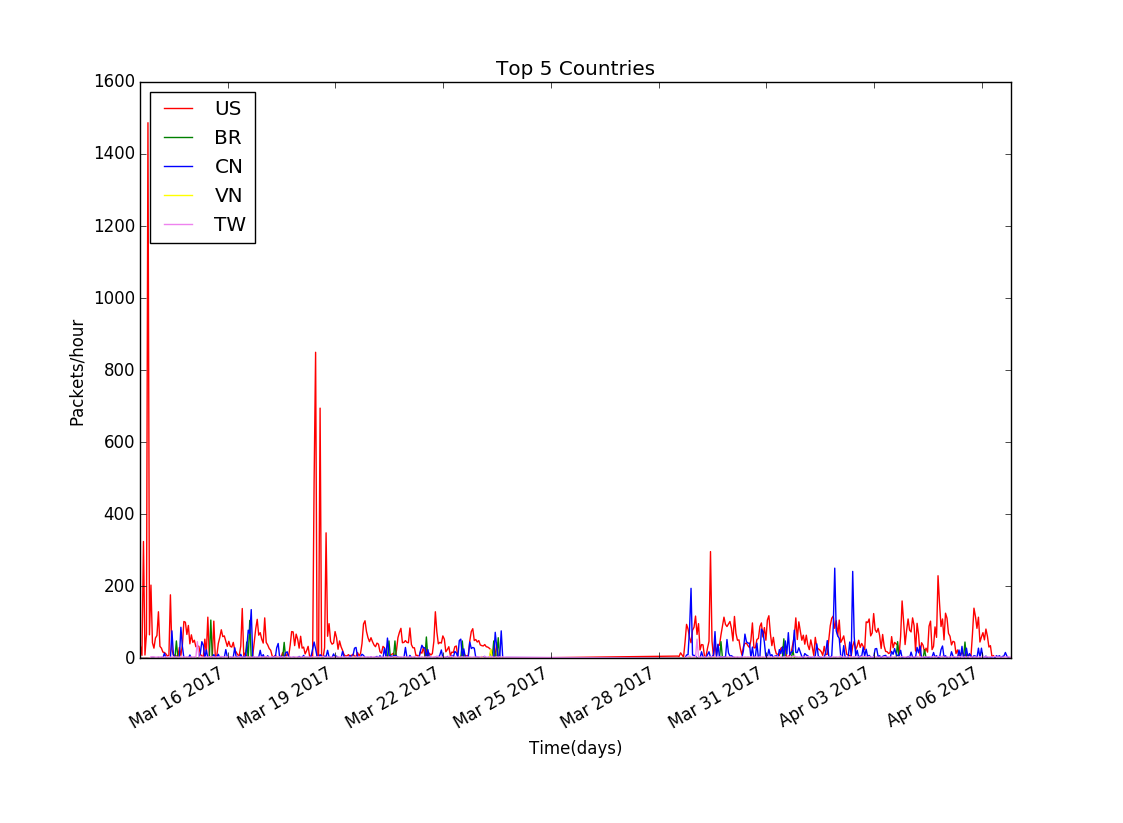
\includegraphics[width=15cm, height=9cm]{images/top5countries_udp_honeypot.png}
\caption{Top 5 countries participated in UDP port scanning activity and its traffic rate (second configuration)}
\end{figure}
\\\\
Figure 7.20 and Figure 7.21 show the graphs of top 5 countries who participated in UDP port scanning activity and its traffic rate based on the local time of the source of attack from first and second configuration respectively.
From these graphs, we can understand that UDP port scans are not very frequent as TCP port scanning activity.
However, UDP port scans do not show a correlation between traffic and time of the day as similar TCP port scanning activity.
Moreover, top 5 countries which are involved in UDP port scans at both first and second configuration are same and are China, United States, Vietnam, Brazil and Taiwan.
Another interesting fact is that, these are the top 5 countries which involved in TCP port scans as well.
\subsection{ Geographical Distribution of Port Scan Sources}
Another property we wanted to check is how port scan source IP addresses are geographically distributed around the world.
We implemented a method to do it by designing a heat map to show the geographical distribution of location of port scanning attacks.
\begin{figure}[p]
\centering
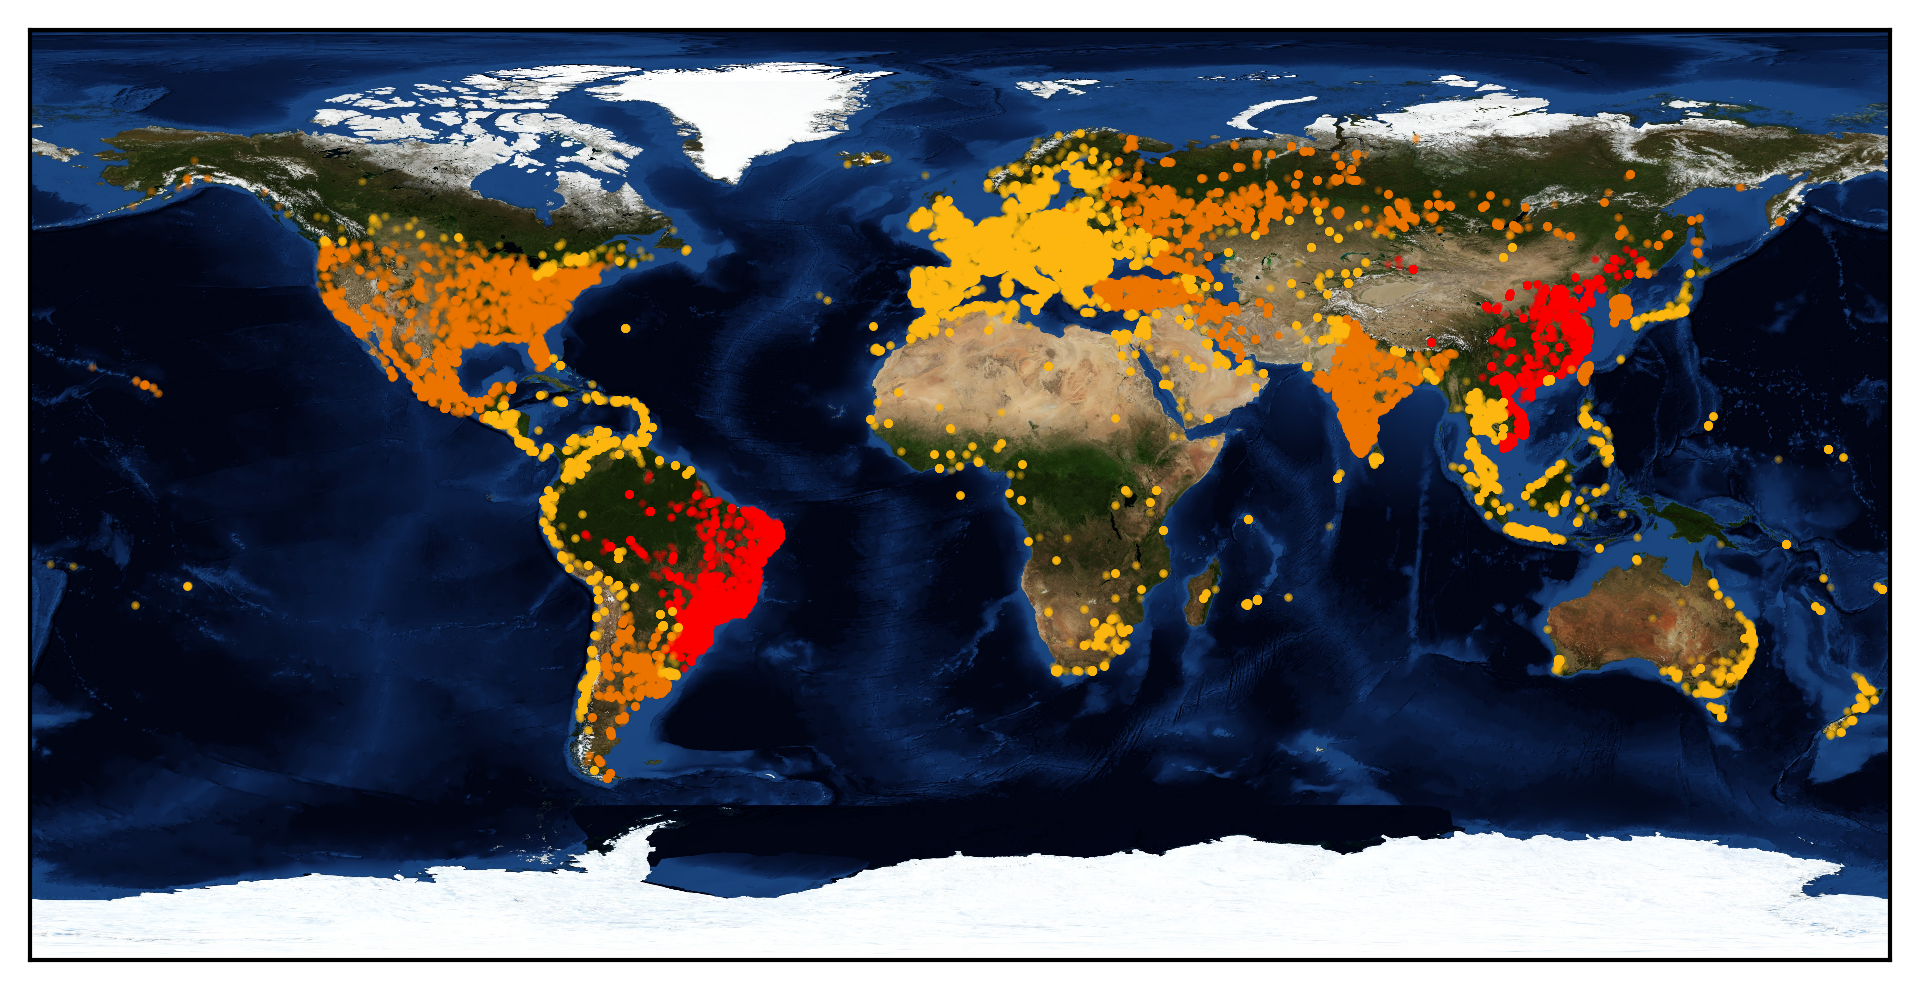
\includegraphics[width=14cm, height=8cm]{images/geographical_jan.png}
\caption{Geographic Distribution of Port Scan Source IP Addresses at First Configuration}
\end{figure}
\begin{figure}[p]
\centering
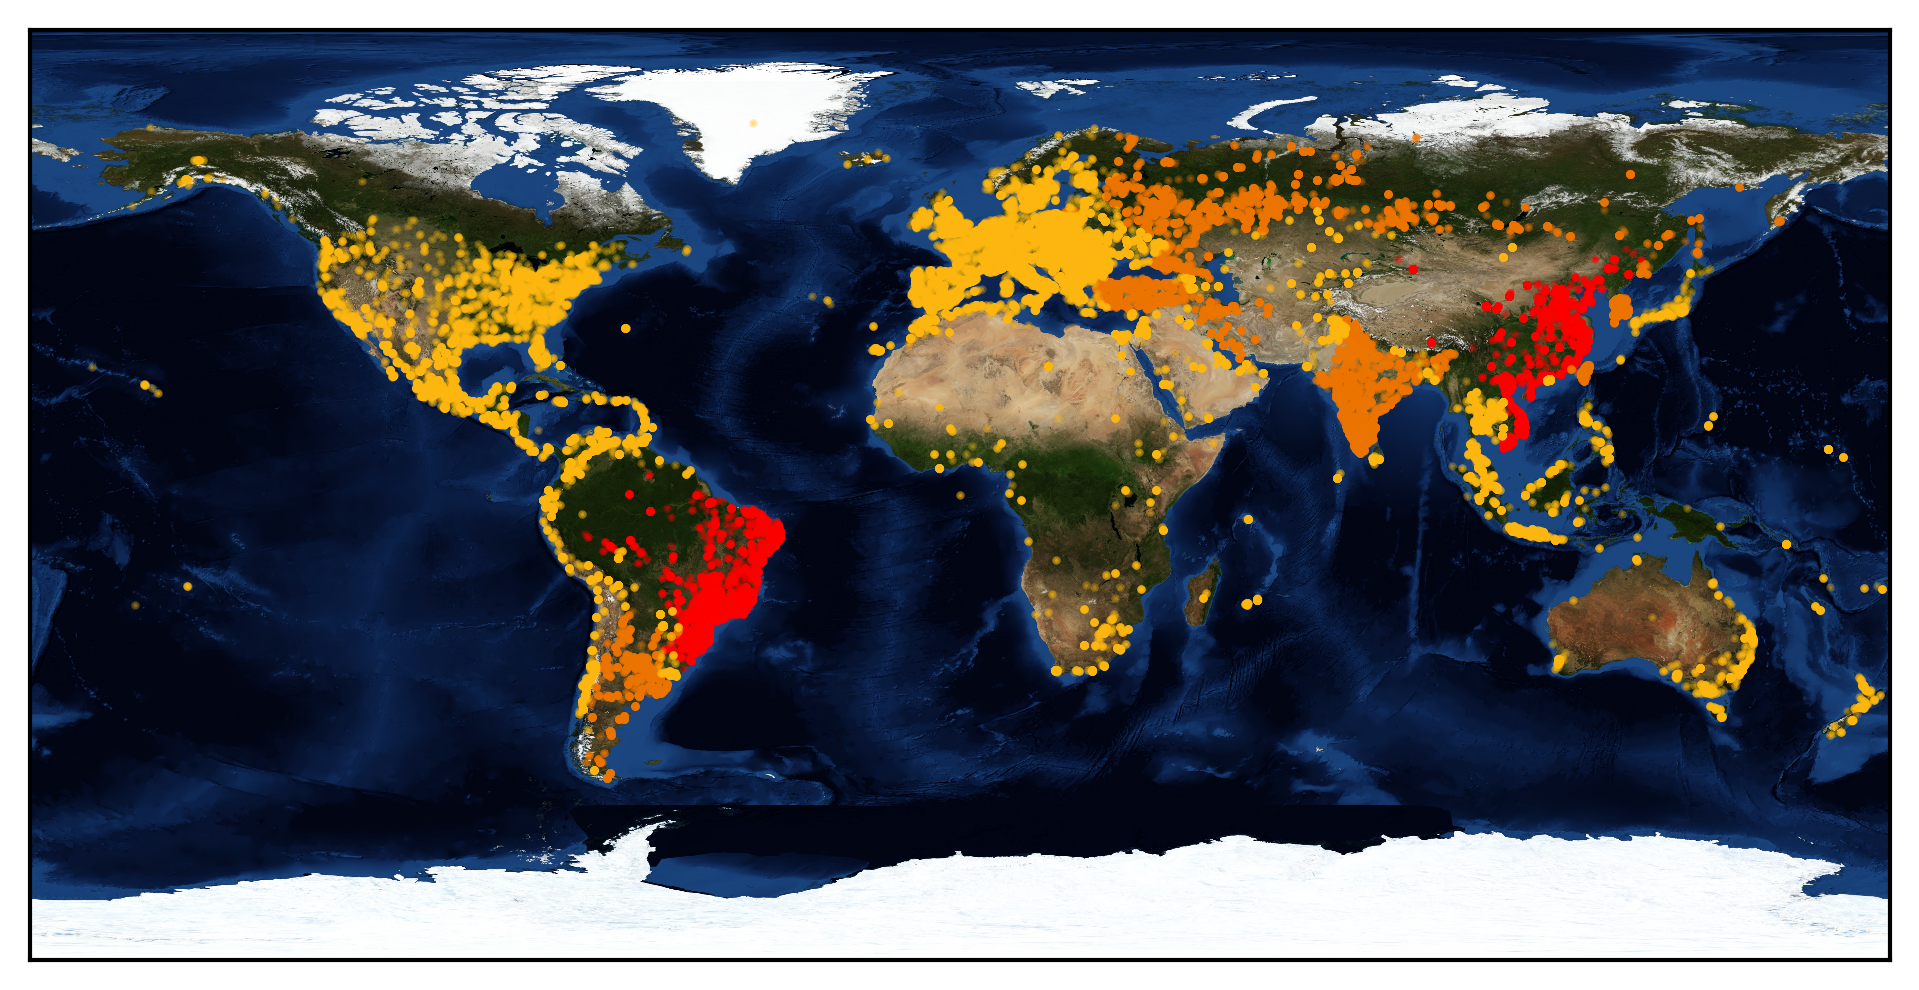
\includegraphics[width=14cm, height=8cm]{images/geographical_march.png}
\caption{Geographic Distribution of Port Scan Source IP Addresses at Second Configuration}
\end{figure}
\\\\ 
Figure 7.22 and Figure 7.23 show the geographical distribution of port scan source IP address at first and second configuration respectively.
These two heat maps show similar behavior in respect to the origin of port scans.
These maps show that port scans are a global phenomena and it originate from a multitude of locations across the world and seem to be correlated only with accessibility of the Internet. 
